\documentclass[a4paper, 10pt]{article}

\usepackage[utf8]{inputenc}
\usepackage[margin=2.5cm, top=3.5cm]{geometry}
\usepackage[spanish]{babel}
\usepackage{graphicx}
\usepackage[hidelinks]{hyperref}
\usepackage{fancyhdr}
\usepackage{lipsum} 
\usepackage{caption}
\usepackage{xcolor}
\usepackage{colortbl}
\usepackage{float}
\usepackage{array}
\usepackage{booktabs}

% Variables
\newcommand{\logoPortada}{images/logo_uni.png}


\pagestyle{fancy}

\fancyhead[L]{\leftmark}    
\fancyhead[C]{}             
\fancyhead[R]{\textcolor{red}{\thepage}}
\fancyfoot{} 



\begin{document}

% -----------------------------------------PORTADA-------------------------------------------------------------
    \begin{titlepage}
        \centering
        \includegraphics[width=0.2\textwidth]{\logoPortada} \par\vspace{1cm}
        {\scshape\LARGE \textbf{Universidad de Sevilla}}\par\vspace{1cm}
        {\scshape\Large ESCUELA TÉCNICA SUPERIOR DE INGENIERÍA INFORMÁTICA}\par\vspace{1cm}
        GRADO EN INGENIERÍA INFORMÁTICA DEL SOFTWARE\par\vspace{1cm}
        TRABAJO FIN DE GRADO\par\vspace{1cm}
        {\huge\bfseries Desarrollo de una auditoría de ciberseguridad para PYMEs}\par\vspace{1cm}
        Realizado por:\par\vspace{0.1cm}
        {\Large\itshape Álvaro Ruiz Gutiérrez}\par\vspace{1cm}
        Dirigido por:\par\vspace{0.1cm}
        {\Large\itshape Alejandro Carrasco Muñoz}\par\vspace{1cm}
        Departamento:\par\vspace{0.1cm}
        {\Large\itshape Tecnología Electrónica}\par\vspace{1cm}
        2024/2025
    \end{titlepage}
    \clearpage
% -----------------------------------------------INDICES------------------------------------------------------------

\tableofcontents
\thispagestyle{empty}
\clearpage


\listoffigures
\thispagestyle{empty}
\clearpage


\listoftables
\thispagestyle{empty}
\clearpage


% -----------------------------------------------AGRADECIMIENTOS------------------------------------------------------------

\section*{Agradecimientos}
\section*{Familiares}

\thispagestyle{empty}

\vfill
\begin{flushright}
\begin{minipage}{0.5\textwidth}
A mi familia, por estar siempre presente en cada paso del camino. Gracias por vuestro amor, comprensión y por haberme dado el apoyo necesario, también en lo económico, para poder continuar con mi formación.
\end{minipage}
\end{flushright}
\clearpage

\section*{Mi pareja y familiares}
\thispagestyle{empty}

\vfill
\begin{flushright}
\begin{minipage}{0.5\textwidth}
A mi novia y a su familia, por su apoyo incondicional y por sostenerme en los momentos más difíciles. Gracias por estar siempre, por el cariño, la paciencia y por motivarme a seguir adelante cuando más lo necesitaba.
\end{minipage}
\end{flushright}
\clearpage

\section*{Mi Tutor}
\thispagestyle{empty}

\vfill
\begin{flushright}
\begin{minipage}{0.5\textwidth}
A mi tutor Alejandro, por aceptar ser parte de este camino. Gracias por la confianza depositada en mí, por las facilidades aportadas y por abrirme la puerta hacia una nueva etapa profesional.
\end{minipage}
\end{flushright}
\clearpage

\section*{BeeHacker}
\thispagestyle{empty}
\vfill
\begin{flushright}
\begin{minipage}{0.5\textwidth}
A la empresa Beehacker, por su colaboración en este proyecto. Agradezco sinceramente la oportunidad que me han ofrecido para aplicar mis conocimientos en un entorno real y su implicación durante todo el proceso.
\end{minipage}
\end{flushright}
\clearpage



% -----------------------------------------------RESUMEN------------------------------------------------------------

\section*{Resumen}
\thispagestyle{empty}
Las pequeñas y medianas empresas (PYMEs) desempeñan un papel importante en la economía global. Sin embargo, su creciente
digitalización ha aumentado su exposición a ciberataques, debido a infraestructuras de seguridad limitadas y con recursos insuficientes para enfrentar amenazas sofisticadas. 
Este proyecto tiene como objetivo principal desarrollar un modelo de auditoría de ciberseguridad adaptado a las PYMEs, basándose en la normativa europea y nacional vigente. Para garantizar su usabilidad, se elaborará una guía accesible para usuarios sin conocimientos técnicos previos, permitiéndoles evaluar la seguridad de sus entornos digitales.
\par\vspace{0.5cm}

El proyecto se divide en dos fases principales. En la primera, se establecerá un marco teórico que explore las herramientas más comunes en auditorías de seguridad, las normativas aplicables y las metodologías más utilizadas en el ámbito de la ciberseguridad. Se examinarán los diferentes tipos de auditorías y se proporcionarán diferentes métodos para mitigar posibles riesgos. Esta fase permitirá comprender en profundidad las vulnerabilidades específicas del entorno empresarial y cómo abordarlas.
\par\vspace{0.5cm}

La segunda fase estará dedicada a la implementación práctica de la auditoría, siguiendo una 
metodología estructurada que abarcará desde el análisis del perímetro de red hasta la evaluación de la seguridad de los datos. 
Se incluirán en el diseño, pruebas en aplicaciones web, dispositivos IoT y la infraestructura interna de la empresa. 
Esta parte culminará con un caso práctico que ilustrará el proceso parcial de una auditoría de ciberseguridad en un entorno real, proporcionando una visión clara de cómo aplicar las técnicas aprendidas.
\par\vspace{0.5cm}

Finalmente, se incluirá un informe profesional que documente de forma detallada tanto el desarrollo del proceso de auditoría como los resultados obtenidos, proporcionando así una visión clara y estructurada del estado de ciberseguridad de la organización evaluada.

\par\vspace{0.5cm}
\textbf{Palabras clave:} ciberseguridad, auditoría, PYMEs, vulnerabilidades, normativas, metodologías, buenas prácticas.
\clearpage

% -----------------------------------------------ABSTRACT------------------------------------------------------------

\section*{Abstract}
\thispagestyle{empty}
Small and medium-sized enterprises (SMEs) play a crucial role in the global economy. However, their increasing digitalization has heightened their exposure to cyberattacks, due to limited security infrastructures and insufficient resources to counter sophisticated threats.
The main objective of this project is to develop a cybersecurity audit model tailored to SMEs, based on current European and national regulations. To ensure usability, an accessible guide will be created for users with no prior technical knowledge, enabling them to assess the security of their digital environments.
\par\vspace{0.5cm}

The project is divided into two main phases. In the first phase, a theoretical framework will be established, exploring the most common tools used in security audits, the applicable regulations, and the most widely used methodologies in the field of cybersecurity. Different types of audits will be examined, and various methods will be provided to mitigate potential risks. This phase will offer a deep understanding of the specific vulnerabilities within business environments and how to address them.
\par\vspace{0.5cm}

The second phase will focus on the practical implementation of the audit, following a structured methodology that covers everything from network perimeter analysis to data security assessment.
The design will include testing in web applications, IoT devices, and the company's internal infrastructure.
This phase will culminate in a practical case study illustrating the partial process of a cybersecurity audit in a real-world environment, offering a clear view of how to apply the techniques learned.
\par\vspace{0.5cm}

Finally, a professional report will be included, documenting in detail both the audit process and the results obtained, thus providing a clear and structured overview of the cybersecurity status of the evaluated organization.
\par\vspace{0.5cm}
\textbf{Keywords:} cybersecurity, audit, SMEs, vulnerabilities, regulations, methodologies, best practices.
\clearpage



% -----------------------------------------------INTRODUCCION------------------------------------------------------------
\section{Introducción}
En el mundo digital actual, la ciberseguridad ya no es una opción, sino una necesidad. Las pequeñas y medianas empresas (PYMEs), pilares fundamentales de la economía global, se encuentran entre los objetivos más vulnerables frente a ciberataques. A pesar de su importancia económica, 
muchas de estas empresas subestiman su exposición a amenazas digitales, creyendo erróneamente que su tamaño las hace pasar desapercibidas para los ciberdelincuentes. Sin embargo, esta percepción es un error crítico, ya que la limitada infraestructura de seguridad de las 
PYMEs las convierte en blancos fáciles. 
\par\vspace{0.5cm}

Un claro ejemplo de la creciente amenaza cibernética es el ataque sufrido por el portal de afiliación del sindicato Comisiones Obreras (CCOO) en diciembre de 2023 \cite{farlopa}. El atacante explotó una vulnerabilidad en el formulario de afiliación, accediendo a la configuración interna del sitio web. Esta brecha permitió la subida de un archivo malicioso que otorgó control total sobre el sistema, facilitando el acceso a información sensible, incluyendo contraseñas sin la protección adecuada. Como resultado, el atacante alteró la página de inicio de aproximadamente 50 subdominios de ccoo.es, demostrando la facilidad con la que se puede comprometer la seguridad digital de una organización.
\par\vspace{0.5cm}

Este incidente subraya la necesidad de fortalecer la ciberseguridad en organizaciones de todos los tamaños. Las PYMEs, en particular, son especialmente susceptibles debido a la escasez de recursos y, en muchos casos, a una falta de concienciación sobre las amenazas digitales. 
La creciente digitalización y la dependencia de sistemas conectados a la red han ampliado la superficie de ataque, exponiendo a estas organizaciones a riesgos significativos.
\par\vspace{0.5cm}

En este contexto, es crucial que las PYMEs adopten medidas proactivas para proteger sus activos digitales. Este trabajo propone una guía práctica para la realización de auditorías de ciberseguridad, con el objetivo de identificar vulnerabilidades, evaluar riesgos y establecer 
estrategias de mitigación efectivas. A través de esta guía, se busca que las PYMEs fortalezcan su seguridad informática y enfrenten con mayor confianza los desafíos del entorno digital actual.

\clearpage



\subsection{Objetivos}

El objetivo principal de este trabajo es dise\~nar un modelo de auditor\'ia de ciberseguridad  espec\'ifico para PYMEs, que sea f\'acil de implementar por personas sin conocimientos t\'ecnicos avanzados. Los objetivos espec\'ificos incluyen:

\begin{itemize}
    \item Establecer un marco te\'orico que contemple las herramientas, t\'ecnicas y normativas actuales en ciberseguridad.
    \item Proponer una metodolog\'ia de auditor\'ia completa y estructurada.
    \item Desarrollar un caso pr\'actico en una PYME real para validar la metodolog\'ia propuesta.
    \item Redactar un informe detallado que incluya el an\'alisis de riesgos, vulnerabilidades detectadas y recomendaciones de mejora.
    \item Elaborar una guía clara y comprensible, diseñada específicamente para ser utilizada por personas sin conocimientos técnicos previos.
\end{itemize}

\subsection{Alcance}

El alcance está diseñado para cubrir todos los aspectos necesarios para realizar una auditoría de ciberseguridad efectiva en PYMEs, basándose en estándares y metodologías reconocidas internacionalmente.

\begin{enumerate}
    \item \textbf{Marco teórico:} Se explorarán las herramientas más utilizadas en auditorías de ciberseguridad, las normativas relevantes tanto a nivel nacional como europeo, los distintos tipos de auditoría existentes y las recomendaciones de organizaciones como OWASP, SANS y OSSTM.
    
    \item \textbf{Requisitos previos:} Se detallarán los conocimientos, habilidades y recursos técnicos necesarios para realizar auditorías efectivas, incluyendo la configuración de entornos de prueba y el uso de herramientas especializadas.
        
    \item \textbf{Propuesta de metodología:} Se desarrollará una metodología estructurada que incluirá el análisis exhaustivo de todos los aspectos a evaluar en una auditoria de ciberseguridad completa. Esta abarcará el perímetro de red, la seguridad inalámbrica, la identificación de vulnerabilidades, pruebas sobre aplicaciones web, evaluación de la infraestructura interna y análisis de seguridad en endpoints y sistemas de almacenamiento de datos.
    
    \item \textbf{Caso práctico:} Se implementará un caso práctico que aplicará la metodología propuesta de manera parcial en un entorno real, permitiendo ilustrar de manera tangible el proceso completo de una auditoría de ciberseguridad.
    
    \item \textbf{Informe final:} Elaboración de un documento que refleje el estado actual de la ciberseguridad en la empresa auditada y las recomendaciones pertinentes.
\end{enumerate}


\subsection{Motivación}
La creciente digitalización ha expuesto a las Pequeñas y Medianas Empresas (PYMEs) a una variedad de ciberamenazas que, de no ser gestionadas adecuadamente, 
pueden poner en riesgo la continuidad de sus operaciones. A diferencia de las grandes corporaciones, las PYMEs suelen carecer de los recursos humanos y financieros 
necesarios para implementar medidas robustas de ciberseguridad, lo que las convierte en un fácil objetivo para los ciberdelincuentes.
\par\vspace{0.5cm}
El aumento en el volumen de software malicioso, que supera los 450.000 nuevos programas diarios \cite{avtest}, y el hecho de que el 70 
por ciento de los ciberataques en la Península Ibérica afectan a PYMEs, subrayan la urgencia de desarrollar herramientas accesibles y eficaces para proteger a estas organizaciones. 
Este proyecto surge como respuesta a esa necesidad, proporcionando una guía práctica que permite a cualquier persona, independientemente de su nivel técnico, llevar a cabo una auditoría 
básica de ciberseguridad.
\par\vspace{0.5cm}
Además, una de las principales motivaciones personales que ha impulsado la realización de este trabajo es mi interés en formarme profesionalmente como pentester. 
Este proyecto representa un primer paso en ese camino, permitiéndome aplicar conocimientos teóricos y prácticos en un entorno real. Al mismo tiempo, me gustaría que esta guía 
pudiera servir como punto de partida para otros estudiantes en prácticas o personas con poca experiencia que deseen introducirse en el ámbito de la ciberseguridad. 
De este modo, no solo se contribuye a la protección de las PYMEs, sino también al desarrollo de nuevos profesionales en el sector.
\par\vspace{0.5cm}


\subsection{Requisitos formales}
Una vez definido el contexto general del trabajo, se establecen los requisitos formales necesarios para la correcta redacción y desarrollo del documento.

\subsubsection{Documentación e información}
\begin{itemize}
    \item Los documentos pueden ser extraídos de \textit{Google Scholar} para su posterior citación.
    \item Se recomienda utilizar publicaciones con una antigüedad no superior a 3 o 4 años, para asegurar la vigencia de la información
    \item Todos los documentos consultados se citarán en formato APA.
    \item Deben contener información relevante y actualizada sobre ciberseguridad en PYMEs.
\end{itemize}

\subsubsection{Normativas y certificaciones}
\begin{itemize}
    \item Deben ser oficiales y de libre acceso, proporcionadas por organismos reguladores tanto de ámbito europeo como internacional.
\end{itemize}

\subsubsection{Propuesta de metodología de la auditoría}
\begin{itemize}
    \item Debe atender a los requerimientos de ciberseguridad descritos en la documentación oficial.
    \item Describir las implementaciones de hardware y software necesarias para proteger los sistemas.
\end{itemize}

\subsubsection{Sobre el caso práctico}
\begin{itemize}
    \item Descripción del sistema auditado, incluyendo modelo y vulnerabilidades.
    \item Aplicación de la metodología de ciberseguridad en la PYME seleccionada.
    \item Detalle de las pruebas realizadas y la obtención de información sobre riesgos, amenazas y vulnerabilidades.
\end{itemize}


\subsection{Estructura del documento}

El documento está organizado en once capítulos que abordan de manera integral todos los aspectos necesarios para realizar una auditoría de ciberseguridad en PYMEs:

\begin{itemize}
    \item \textbf{Agradecimientos:} Reconocimiento a las personas y entidades que han contribuido al desarrollo de este trabajo.
    
    \item \textbf{Resumen:} Síntesis del contenido, objetivos y resultados del trabajo.
    
    \item \textbf{Introducción:} Presentación del contexto de la ciberseguridad en PYMEs, objetivos, alcance, motivación, requisitos formales para el desarrollo del proyecto y estructura del documento.
    
    \item \textbf{Planificación:} Descripción de la organización del trabajo, incluyendo cronograma, recursos utilizados, costes y fases del proyecto.
    
    \item \textbf{Marco Teórico (Estado del arte):} Análisis de normativas nacionales y europeas aplicables, estándares, herramientas de pentesting y técnicas relevantes en el ámbito de la ciberseguridad para PYMEs.
    
    \item \textbf{Requisitos:} Definición de los requisitos técnicos, necesarios para llevar a cabo una auditoría de seguridad.
    
    \item \textbf{Modelo de auditoría:} Propuesta de un modelo de auditoría dividido en diseño, metodología y fases específicas.
    
    \item \textbf{Caso Práctico:} Implementación de la auditoría en un entorno real de una PYME, aplicando las herramientas y técnicas descritas.
    
    \item \textbf{Resultados:} Presentación y análisis de los resultados obtenidos en el caso práctico.
    
    \item \textbf{Conclusión:} Reflexión sobre los hallazgos, lecciones aprendidas y posibles trabajos futuros.
    
    \item \textbf{Referencias:} Fuentes consultadas para la realización del trabajo.
    
    \item \textbf{Anexos:}  Material complementario que apoya el desarrollo del caso práctico y la comprensión de la metodología.

\end{itemize}




\clearpage

% -----------------------------------------------PLANIFICACION------------------------------------------------------------
\section{Planificación}
Este capítulo presenta la planificación detallada para el desarrollo del trabajo. Se describirán las fases y tareas específicas a desarrollar, los roles y responsabilidades de los participantes en el proyecto, así como un cronograma que permitirá visualizar el progreso del trabajo a lo largo del tiempo. Además, se identificarán los recursos necesarios para llevar a cabo el proyecto y se realizará un análisis de los costes asociados.

\subsection{Fases y lista de actividades}
\par\vspace{0.5cm}
\textbf{\large Fase 1 - Gestión del Proyecto} \vspace{0.5cm}

\begin{itemize}
    \item \textbf{1.1 Plan de Inicio}
    \begin{itemize}
        \item \textbf{1.1.1 Reunión inicial:} Primer encuentro con el tutor para explorar posibles temas de interés para el TFG.
        \item \textbf{1.1.2 Investigación preliminar:} Análisis de las diferentes opciones y selección del tema más adecuado.
        \item \textbf{1.1.3 Adjudicación TFG:} Confirmación oficial del tema y asignación del trabajo.
        \item \textbf{1.1.4 Inicio del trabajo:} Comienzo formal de la redacción y desarrollo del trabajo.
        \item \textbf{1.1.5 Investigación orientada a los objetivos:} Ampliación del conocimiento sobre el tema seleccionado.
        \item \textbf{1.1.6 Segunda reunión con el tutor:} Reunión para debatir la estructura y organización del TFG.
        \item \textbf{1.1.7 Reunión con CTO BeeHacker:} Análisis de la viabilidad del trabajo y perspectivas del sector.
        \item \textbf{1.1.8 Segunda reunión con CTO BeeHacker:} Obtención de información adicional.
        \item \textbf{1.1.9 Desarrollo de la introducción:} Definición clara de los objetivos, alcance, motivación y requisitos.
        \item \textbf{1.1.10 Revisión de la introducción:} Revisión y aprobación del plan de inicio.
    \end{itemize}

    \item \textbf{1.2 Planificación}
    \begin{itemize}
        \item \textbf{1.2.1 Definición de fases y tareas:} Establecimiento de las fases y actividades del proyecto.
        \item \textbf{1.2.2 Definición de roles y responsables:} Asignación de roles y responsabilidades del proyecto.
        \item \textbf{1.2.3 Cronograma:} Desarrollo del cronograma en MSProject.
        \item \textbf{1.2.4 Recursos:} Identificación de recursos humanos y materiales.
        \item \textbf{1.2.5 Estimación de costes:} Cálculo del presupuesto estimado.
        \item \textbf{1.2.6 Revisión de la planificación:} Revisión y aprobación de la planificación.
    \end{itemize}

    \item \textbf{1.3 Seguimiento y Control}
    \begin{itemize}
        \item \textbf{1.3.1 Corrección de la introducción:} Corrección y ajuste de la introducción.
        \item \textbf{1.3.2 Corrección de la planificación:} Corrección y ajuste de la planificación.
        \item \textbf{1.3.3 Corrección del marco teórico:} Corrección y ajuste del marco teórico.
        \item \textbf{1.3.4 Corrección del modelo de auditoría:} Corrección y ajuste del modelo de auditoría.
        \item \textbf{1.3.5 Informe y control del desempeño:} Generación de informes de seguimiento.
    \end{itemize}

    \item \textbf{1.4 Cierre}
    \begin{itemize}
        \item \textbf{1.4.1 Informe final con resultados:} Documentación final con las conclusiones.
        \item \textbf{1.4.2 Plan de mitigación de riesgos:} Propuesta de acciones correctivas.
        \item \textbf{1.4.3 Lecciones aprendidas:} Reflexión sobre los conocimientos adquiridos.
    \end{itemize}
\end{itemize}

\vspace{0.5cm}
\textbf{\large Fase 2 - Desarrollo del Producto} \vspace{0.5cm}

\begin{itemize}
    \item \textbf{2.1 Marco teórico}
    \begin{itemize}
        \item \textbf{2.1.1 Desarrollo del marco teórico:} Investigación, análisis, redacción y estructuración del marco conceptual.
        \item \textbf{2.1.2 Revisión del marco teórico:} Revisión y aprobación del marco teórico.
    \end{itemize}

    \item \textbf{2.2 Modelo de auditoría}
    \begin{itemize}
        \item \textbf{2.2.1 Diseño del modelo:} Definición de la estructura metodológica y los procedimientos a seguir.
        \item \textbf{2.2.2 Revisión del modelo:} Revisión y aprobación del modelo de auditoría.
    \end{itemize}

    \item \textbf{2.3 Caso práctico}
    \begin{itemize}
        \item \textbf{2.3.1 Desarrollo del caso práctico:} Ejecución y aplicación en la PYME.
        \item \textbf{2.3.2 Seguimiento de la práctica:} Monitorización y análisis del proceso.
    \end{itemize}
\end{itemize}

\vspace{0.5cm}
\textbf{\large Fase 3 - Revisión técnica formal} \vspace{0.5cm}

\begin{itemize}
    \item \textbf{3.1 Revisión del proyecto}
    \begin{itemize}
        \item \textbf{3.1.1} Análisis completo del trabajo desarrollado y correcciones necesarias.
    \end{itemize}
\end{itemize}

\vspace{0.5cm}
\textbf{\large Fase 4 - Presentación} \vspace{0.5cm}

\begin{itemize}
    \item \textbf{4.1 Presentación del proyecto}
    \begin{itemize}
        \item \textbf{4.1.1} Exposición y defensa del trabajo realizado.
    \end{itemize}
\end{itemize}




\subsection{Roles y responsabilidades}

\begin{table}[H]
    \centering
    \caption{Distribución de roles y responsabilidades en el proyecto}
    \begin{tabular}{|c|c|}

        \hline
        \textbf{Rol} & \textbf{Responsabilidad} \\
        \hline
        Analista/Desarrollador (Alumno) & Planificación y redacción del documento \\
        \hline
        Analista/Desarrollador (Alumno) & Investigación y análisis de ciberseguridad en PYMEs \\
        \hline
        Analista/Desarrollador (Alumno) & Desarrollo del marco teórico \\
        \hline
        Analista/Desarrollador (Alumno) & Agrupación y redacción de requisitos previos para auditoría \\
        \hline
        Analista/Desarrollador (Alumno) & Identificación y documentación de normativas aplicables \\
        \hline
        Analista/Desarrollador (Alumno) & Creación de plan de auditoría propio \\
        \hline
        Analista/Desarrollador (Alumno) & Diseño de la metodología de auditoría \\
        \hline
        Analista/Desarrollador (Alumno) & Implementación práctica de la auditoría \\
        \hline
        Analista/Desarrollador (Alumno) & Ejecución del caso práctico \\
        \hline
        Analista/Desarrollador (Alumno) & Análisis de resultados y redacción del informe final \\
        \hline
        Jefe de proyecto (Tutor) & Asesoramiento en la selección del tema y enfoque del proyecto \\
        \hline
        Jefe de proyecto (Tutor) & Orientación y supervisión del trabajo del alumno \\
        \hline
        Jefe de proyecto (Tutor) & Organizar el desarrollo del caso práctico \\
        \hline
        Jefe de proyecto (Tutor) & Correcciones y evaluación del proyecto \\
        \hline
        Jefe de equipo (CTO de BeeHacker) & Proporcionar información técnica relevante y feedback \\
        \hline
        Jefe de equipo (CTO de BeeHacker) & Validación de la metodología y resultados del caso práctico \\
        \hline

    \end{tabular}
    \begin{flushleft}\centering
        \footnotesize \textbf{Fuente:} Elaboración propia
    \end{flushleft}    
    \label{tab:distribucion_roles}
\end{table}



\subsection{Cronograma}
ANALISIS FINAL CON EL MSProject

\subsection{Recursos}

Los recursos necesarios para el desarrollo de la auditoría de ciberseguridad se dividen en tres categorías principales: recursos humanos, materiales y costos asociados. A continuación, se detallan cada uno de ellos.

\subsubsection{Recursos Humanos}

En virtud del documento oficial de la Agencia Digital de Andalucía \cite{agencia_digital}, se establecen los costes por hora de los perfiles profesionales necesarios para la realización del proyecto.

\begin{table}[H]
\caption{Recursos Humanos}
\centering
\renewcommand{\arraystretch}{1.5}
\begin{tabular}{|c|c|c|}
\hline
\textbf{Recurso} & \textbf{Tipo} & \textbf{Costo por Hora}  \\ \hline
Director de Proyecto & Trabajo & 63,75 €/h  \\ \hline
Jefe de Equipo & Trabajo & 53,55 €/h  \\ \hline
Analista & Trabajo & 47,17 €/h  \\ \hline
\end{tabular}
\begin{flushleft}\centering
    \footnotesize \textbf{Fuente:} Elaboración propia
\end{flushleft}   
\label{tab:recursos_humanos}
\end{table}



\subsubsection{Recursos Materiales}
\begin{table}[H]
\caption{Recursos Materiales}
\centering
\renewcommand{\arraystretch}{1.5}
\begin{tabular}{|c|c|c|c|c|}
\hline
\textbf{Recurso} & \textbf{Tipo} & \textbf{Costo Unitario} & \textbf{Unidades} & \textbf{Costo Total}  \\ \hline
Impresora & Material & €50,00 & 1& €50,00  \\ \hline
Disco Duro Externo & Material &  €60,00 &1& €60,00  \\ \hline
Pen Drive & Material & €20,00 & 1& €20,00  \\ \hline
Ordenador & Material & €600,00 & 1& €600,00  \\ \hline
Herramientas Hacking & Material & €500,00 & 1& €500,00  \\ \hline
\end{tabular}
\begin{flushleft}\centering
    \footnotesize \textbf{Fuente:} Elaboración propia
\end{flushleft}   
\label{tab:recursos_materiales}
\end{table}



\subsubsection{Costos Asociados}

\begin{table}[H]
\caption{Costos Asociados}
\centering
\renewcommand{\arraystretch}{1.5}
\begin{tabular}{|c|c|c|c|}
\hline
\textbf{Recurso} & \textbf{Tipo} & \textbf{Costo Total} & \textbf{Coste Estimado}  \\ \hline
Reserva de Contingencia & Costo & Variable & 1000€  \\ \hline
Licencias Software & Costo & Variable &  100€ \\ \hline
\end{tabular}
\begin{flushleft}\centering
    \footnotesize \textbf{Fuente:} Elaboración propia
\end{flushleft}   
\label{tab:costos_asociados}
\end{table}



\subsection{Estimación de Costes}

Considerando los recursos descritos anteriormente, se prevé que el \textbf{Analista} desempeñe un total de \textbf{300 horas de trabajo}, lo que supone un coste estimado de \underline{14.151 €}.  
\par\vspace{0.3cm}

En cuanto al \textbf{Director de Proyecto}, se estima una dedicación de \textbf{20 horas} centradas en tareas de corrección, revisión y supervisión general del proyecto, lo que representa un coste de \underline{1.275 €}.  
\par\vspace{0.3cm}

Respecto al \textbf{Jefe de Equipo}, se calcula un total de \textbf{10 horas} destinadas a la asistencia técnica y apoyo en el desarrollo de la auditoría, con un coste asociado de \underline{535,50 €}.  
\par\vspace{0.3cm}

Además, es necesario considerar los \textbf{costos adicionales asociados} al proyecto, entre los que destacan una \textbf{reserva de contingencia} de \underline{1.000 €} para posibles imprevistos y el coste de las \textbf{licencias de software} necesarias, estimado en 100 €, lo que suma un total de \underline{1.100 €}.  
\par\vspace{0.3cm}

En lo que respecta a los \textbf{recursos materiales}, se ha calculado un coste global de \underline{1230 €}, correspondiente a la adquisición de los elementos físicos indispensables para el desarrollo del trabajo.  
\par\vspace{0.3cm}

Este cálculo corresponde a una \textbf{duración estimada del proyecto de 4 meses}, durante los cuales se prevé que los profesionales involucrados realicen las tareas planificadas dentro de las horas estipuladas.  

\par\vspace{0.5cm}
\textbf{De esta manera, los costes totales estimados son los siguientes:}  

\begin{table}[H]
\caption{Resumen de costes del proyecto}
\centering
\renewcommand{\arraystretch}{1.5}
\begin{tabular}{|c|c|}
\hline
\textbf{Concepto} & \textbf{Monto (€)} \\ \hline
Recursos Humanos & 15.961,50 € \\ \hline
Recursos Materiales & 1230 € \\ \hline
Costos Asociados & 1.100 € \\ \hline
\textbf{Total Estimado} & \underline{\textbf{18.291,50 €}} \\ \hline
\end{tabular}
\begin{flushleft}\centering
    \footnotesize \textbf{Fuente:} Elaboración propia
\end{flushleft}   
\label{tab:resumen_costes}
\end{table}



\clearpage































% -----------------------------------------------MARCO TEÓRICO------------------------------------------------------------
\section{Fundamentos básicos de Ciberseguridad}


El presente marco teórico tiene como objetivo establecer una base sólida sobre los principios fundamentales de la ciberseguridad aplicados al contexto de las pequeñas y medianas empresas (PYMEs). A lo largo del capítulo se abordarán los principales riesgos y amenazas que enfrentan estas organizaciones en el entorno digital, así como los marcos regulatorios y normativas más relevantes, tanto a nivel nacional como europeo.

\par\vspace{0.5cm}

Posteriormente, se describen las metodologías de auditoría más reconocidas. También se incluye un apartado dedicado a los planes de mitigación, con el fin de exponer estrategias prácticas frente a las principales vulnerabilidades.

\par\vspace{0.5cm}

Para complementar el enfoque teórico, se introducen las certificaciones profesionales más importantes para quien desee especializarse en ciberseguridad ofensiva (Red Team), así como una recopilación actualizada de las herramientas de pentesting más empleadas en el sector.

\par\vspace{0.5cm}

\par\vspace{0.5cm}

Finalmente, se exponen buenas prácticas abordadas desde una doble perspectiva: por un lado, la del auditor y por otro, la de la empresa auditada.
La exposición de estas bases conceptuales y técnicas da paso a la formulación de una propuesta de auditoría específica para PYMEs, enfocada en mejorar su seguridad digital.
















\subsection{Principales amenazas y riesgos para PYMEs}

La ciberseguridad representa un desafío importante para muchas pequeñas y medianas empresas españolas. Según el informe de Hiscox, cerca del 50\% de las empresas en España sufrió algún tipo de ciberataque en 2023. Las PYMEs, en particular, son cada vez más objetivo de estos ataques debido a su limitada preparación en ciberseguridad. De hecho, solo el 61\% de las empresas con menos de 250 empleados se sienten seguras de su preparación en este sector. \cite{hiscox}
\par\vspace{0.5cm}

El Instituto Nacional de Ciberseguridad (INCIBE) registró en 2022 un total de 118.000 incidentes de ciberseguridad, un 9\% más que el año anterior. Una gran parte de estos incidentes afectaron a pequeñas y medianas empresas, y uno de cada tres se trató de una filtración de datos.\cite{incibe2023}
\par\vspace{0.5cm}

Aunque cada vez más PYMEs aumentan sus presupuestos en ciberseguridad y colaboran con empresas especializadas, muchas todavía optan por contratar a otras empresas especializadas para que se encarguen de gestionar sus servicios de ciberseguridad, 
por falta de personal y recursos internos. Esta 
externalización, debe complementarse con una adecuada cultura interna de seguridad, especialmente mediante la formación del personal.
\par\vspace{0.5cm}

Según PwC España, el 86\% de las organizaciones considera que sus empleados carecen de una cultura de ciberseguridad adecuada, lo que pone en pie la necesidad urgente de concienciación.\cite{pow}
\par\vspace{0.5cm}

Entre las principales ciberamenazas que afectan a las PYMEs según la empresa de Software Treyder \cite{treider} se encuentran:

\begin{itemize}
    \item \textbf{Malware:}  
    El término engloba todo tipo de software malicioso diseñado para infiltrarse o dañar un sistema sin el consentimiento del usuario. Incluye virus, troyanos, spyware y especialmente ransomware, que cifra los datos del sistema y exige un rescate económico para su recuperación. Las PYMEs suelen ser víctimas de malware distribuido por correos adjuntos infectados o a través de enlaces maliciosos en páginas aparentemente legítimas. Además del daño económico, el malware puede provocar la pérdida permanente de datos, el control remoto de equipos y el espionaje corporativo.
\end{itemize}

\vspace{0.5cm}

La relevancia del malware como una de las principales ciberamenazas se refleja claramente en su evolución histórica. Tal y como muestra el informe de AV-TEST, la cantidad total de software malicioso (malware) y aplicaciones potencialmente no deseadas (PUA) ha experimentado un crecimiento exponencial en las últimas décadas, superando en 2024 los 1.500 millones de muestras registradas a nivel mundial. Este aumento constante evidencia que las amenazas digitales siguen sofisticándose y expandiéndose, afectando por igual a grandes empresas y a pequeñas organizaciones como las PYMEs.

\vspace{0.3cm}

\begin{figure}[H]
    \centering
    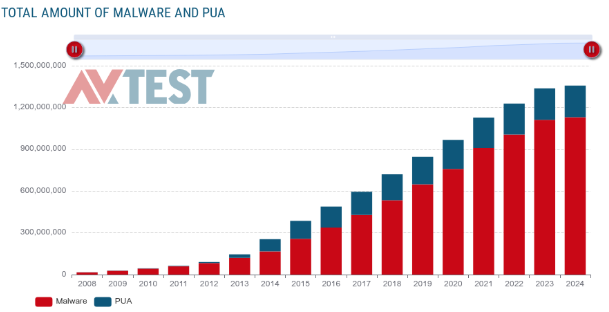
\includegraphics[width=0.95\textwidth]{images/malware.png}
    \caption{Evolución histórica de la cantidad total de malware y PUA a nivel mundial. Fuente: av-atlas.org \cite{avtest}.}
\end{figure}

\vspace{0.5cm}

Aparte del malware, existen otras amenazas igualmente relevantes para las PYMEs:

\begin{itemize}
    \item \textbf{Phishing:}  
    Consiste en técnicas de suplantación de identidad para engañar y obtener datos confidenciales, como contraseñas, credenciales bancarias o información sensible de clientes. Suele realizarse mediante correos electrónicos o mensajes falsificados que imitan a bancos, plataformas de pago o servicios tecnológicos conocidos. En las PYMEs, donde el nivel de concienciación en ciberseguridad suele ser limitado, el phishing representa una puerta de entrada frecuente a ataques más complejos, como el acceso remoto a sistemas o la instalación de malware.
    \vspace{0.3cm}

    \item \textbf{Ataques de denegación de servicio (DDoS):}  
    Este tipo de ataque busca hacer que los servidores, aplicaciones o sitios web de una empresa queden inoperativos mediante el envío masivo de peticiones falsas. Se trata de una sobrecarga intencionada de los recursos tecnológicos de la organización, que impide el funcionamiento normal de servicios clave. Aunque muchas veces se asocian a grandes empresas, las PYMEs también son objetivo, especialmente si ofrecen servicios digitales o tiendas online. Un DDoS puede paralizar las operaciones durante horas o días, con pérdidas económicas importantes y daño reputacional.
    \vspace{0.3cm}

    \item \textbf{Brechas de datos:}  
    Ocurren cuando un atacante consigue acceder sin autorización a bases de datos internas, habitualmente mediante credenciales robadas, vulnerabilidades no parcheadas o ingeniería social. Estas brechas pueden afectar a información crítica como datos de clientes, contraseñas, información financiera o planes estratégicos. Para una PYME, una brecha de datos no solo puede suponer sanciones legales (por ejemplo, si no cumple con el Reglamento General de Protección de Datos (RGPD)), sino también pérdida de confianza por parte de clientes y socios.
    \vspace{0.3cm}

    \item \textbf{Errores de configuración:}  
    Son fallos humanos o técnicos al configurar correctamente sistemas, redes o aplicaciones. Por ejemplo, dejar puertos abiertos innecesarios, permitir contraseñas por defecto, o no establecer permisos adecuados. Estos errores abren puertas invisibles a los ciberatacantes y son especialmente comunes en entornos donde no existe un departamento de TI dedicado. La falta de mantenimiento o revisión de estas configuraciones puede convertir una infraestructura aparentemente segura en un objetivo fácil.

\end{itemize}



\par\vspace{0.5cm}
Además de los vectores de ataques mencionados anteriormente, existen ciertos \textbf{riesgos estructurales} que afectan especialmente a las PYMEs y que incrementan su vulnerabilidad frente a ciberataques:

\begin{itemize}
  \item \textbf{Falta de recursos de seguridad:} Muchas pequeñas empresas no cuentan con personal especializado en ciberseguridad (como un CISO o un técnico en protección de datos), lo que dificulta la detección y respuesta ante incidentes.
  \item \textbf{Presupuestos limitados:} La inversión en ciberseguridad suele ser muy pobre frente a otras prioridades de negocio, lo que impide implementar soluciones de protección efectivas o actualizadas.
  \item \textbf{Falta de diseño seguro desde el inicio:} Al haber sido creadas por expertos en su sector y no por especialistas en tecnología, muchas PYMEs han desarrollado sus sistemas sin tener en cuenta principios de seguridad por defecto.
  \item \textbf{Ausencia de fondos de emergencia:} La falta de capacidad económica para hacer frente a pagos por rescates o pérdidas prolongadas de ingresos hace que las consecuencias de un ciberataque sean especialmente devastadoras.
  \item \textbf{Impacto operativo total ante incidentes graves:} Un ciberataque que provoque una filtración o la caída de sistemas puede detener completamente la actividad del negocio, ya que las PYMEs no suelen tener infraestructuras de respaldo.
\end{itemize}

\par\vspace{0.5cm}
Estos factores, sumados a una falsa sensación de anonimato (“somos demasiado pequeños para que nos ataquen”), aumentan considerablemente el riesgo de que las PYMEs se conviertan en blancos frecuentes y exitosos de los ciberdelincuentes. 
Implementar medidas preventivas y desarrollar una cultura de seguridad sólida resulta crucial para garantizar su continuidad.\cite{toms2021}
\par\vspace{0.5cm}

Finalmente, para ilustrar en tiempo real la magnitud y frecuencia global de estos ataques y reforzar la importancia de adoptar medidas proactivas, puede consultarse el mapa 
interactivo, donde se muestran los ciberataques que se acontecen en tiempo real, proporcionado por Fortinet. 

\begin{figure}[H]
    \centering
    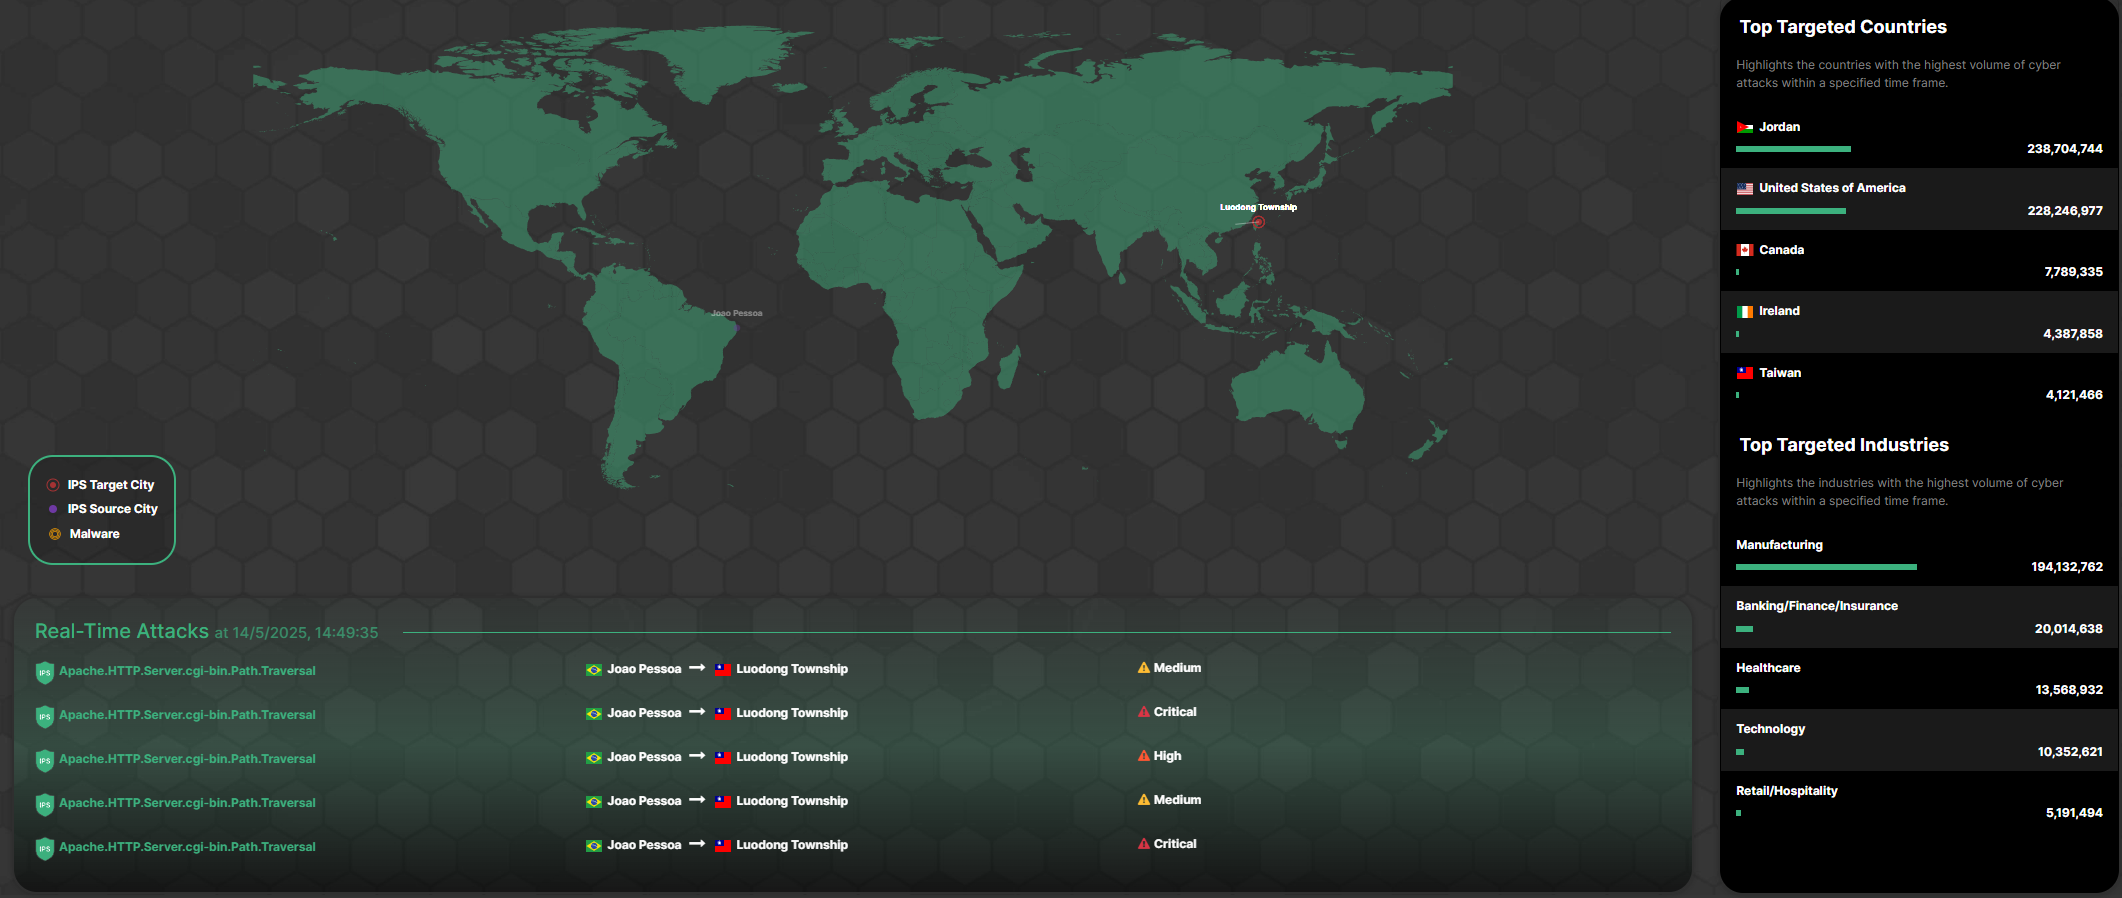
\includegraphics[width=\textwidth]{images/mapa.png}
    \caption{Mapa global de ciberamenazas en tiempo real. Fuente: https://fortiguard.fortinet.com/threat-map}
    \label{fig:mapa-fortiguard}
\end{figure}


\subsection{Normativas nacionales aplicables}

En el contexto español, la legislación vigente en materia de ciberseguridad establece un conjunto de normas esenciales que las PYMEs deben tener en cuenta para garantizar la protección de sus sistemas y datos. Estas normativas buscan no solo proteger la información sensible de las organizaciones, sino también fomentar una cultura de prevención y resiliencia ante los ciberataques.
\par\vspace{0.5cm}

Una de las normativas más relevantes es el \textbf{Esquema Nacional de Seguridad (ENS)}, regulado por el Real Decreto 311/2022. Este marco establece los principios básicos y requisitos mínimos necesarios para una protección adecuada de la información manejada por medios electrónicos, y es de obligado cumplimiento para las entidades del sector público y recomendable para las empresas privadas. El ENS promueve un enfoque basado en riesgos y establece diferentes niveles de seguridad en función del impacto que una amenaza pueda tener sobre la organización. \cite{boe}
\par\vspace{0.5cm}

Asimismo, el \textbf{Real Decreto-ley 12/2018}, sobre seguridad de las redes y sistemas de información, incorpora al derecho español la Directiva NIS de la Unión Europea. Este decreto impone obligaciones a los operadores de servicios esenciales y proveedores de servicios digitales para garantizar un nivel adecuado de seguridad en sus operaciones, además de establecer la necesidad de notificar los incidentes de seguridad más relevantes a la autoridad competente. \cite{boe}
\par\vspace{0.5cm}

Otra normativa destacable es la \textbf{Ley Orgánica 3/2018, de Protección de Datos Personales y garantía de los derechos digitales (LOPDGDD)}, que adapta el Reglamento General de Protección de Datos (RGPD) al ordenamiento jurídico español. Esta ley establece obligaciones específicas en cuanto al tratamiento, almacenamiento y seguridad de los datos personales, lo cual es especialmente relevante en escenarios donde se procesan grandes volúmenes de datos sensibles. \cite{boe}
\par\vspace{0.5cm}

Además, organismos nacionales como el \textbf{Instituto Nacional de Ciberseguridad (INCIBE)} y el \textbf{Centro Criptológico Nacional (CCN)}  han reforzado su colaboración para coordinar acciones frente a las ciberamenazas que afectan tanto a ciudadanos como a empresas, 
proporcionan directrices, guías técnicas y herramientas de apoyo que complementan el cumplimiento normativo, 
especialmente adaptadas a las capacidades de las pequeñas y medianas empresas. \cite{escudo2023}
\par\vspace{0.5cm}

Otra institución fundamental en el ámbito nacional es la \textbf{Agencia Española de Protección de Datos (AEPD)}, organismo encargado de supervisar el cumplimiento de la legislación en materia de privacidad y tratamiento de datos personales. Además, ofrece orientación a empresas y ciudadanos sobre cómo gestionar la información personal de forma segura y responsable.


\subsection{Normativas europeas aplicables}

La Unión Europea ha desarrollado un marco normativo sólido para fortalecer la ciberseguridad en sus Estados miembros, afectando directamente a las PYMEs. Estas regulaciones buscan establecer un nivel común de seguridad y resiliencia operativa en el entorno digital europeo.
\par\vspace{0.5cm}

Una pieza clave es la \textbf{Directiva NIS2} (Directiva (UE) 2022/2555), que entró en vigor en enero de 2023. Esta directiva amplía el alcance de su predecesora, la Directiva NIS, imponiendo requisitos de seguridad más estrictos y procesos de notificación de incidentes más concretos. Se aplica a medianas y grandes empresas de sectores críticos, incluyendo energía, transporte, salud y administración pública. Las empresas deben implementar políticas de gestión de riesgos, autenticación multifactor y formación en ciberseguridad para empleados. \cite{cadena_ser}
\par\vspace{0.5cm}

Otra regulación relevante es el \textbf{Reglamento DORA} (Reglamento (UE) 2022/2554), que establece un marco para la resiliencia operativa digital del sector financiero. Su objetivo es garantizar que todas las entidades financieras puedan soportar, responder y recuperarse de incidentes relacionados con las TIC, asegurando la estabilidad del sistema financiero europeo.\cite{bce}
\par\vspace{0.5cm}

Además, la propuesta de la \textbf{Ley de Ciberresiliencia} de la UE, presentada en septiembre de 2022, busca introducir requisitos horizontales obligatorios de ciberseguridad para productos con elementos digitales, garantizando que los consumidores y empresas puedan confiar en productos digitales seguros. \cite{comision_europea}



\subsection{Metodologías de Auditoría}

Para la realización de los diferentes test que componen la auditoría técnica, se emplean metodologías ampliamente reconocidas en el sector, las cuales proporcionan un marco estructurado y estandarizado para evaluar la seguridad de los sistemas:

\begin{itemize}
  \item \textbf{OWASP (Open Web Application Security Project)}: Enfocada en seguridad de aplicaciones web, sus guías son fundamentales para desarrolladores y auditores.
  \item \textbf{SANS (SysAdmin Audit, Networking and Security Institute)}: Referencia global en formación, certificación y respuesta a incidentes.
  \item \textbf{OSSTM (Open Source Security Testing Methodology Manual)}: Marco metodológico abierto para pruebas de seguridad técnicas, especialmente orientado a entornos éticos y profesionales.
  \item \textbf{NIST 800-82}: Centrada en la seguridad de sistemas de control industrial (ICS, SCADA, DCS, PLC).
  \item \textbf{TIBER-EU}: Framework europeo para pruebas controladas de Red Teaming basadas en inteligencia de amenazas.
\end{itemize}


    \subsection{Planes de Mitigación}

    Para reducir los riesgos derivados de incidentes de ciberseguridad, es fundamental contar con planes de mitigación bien estructurados, 
    que contemplen diversas medidas técnicas y organizativas. 
    Entre las estrategias más efectivas destacan el uso de \textbf{firewalls y filtros de red}, que actúan como barreras de 
    protección frente a accesos no autorizados; el \textbf{monitoreo continuo de red}, que permite la detección temprana de comportamientos anómalos; 
    y la \textbf{protección frente a ataques DDoS}, que asegura la disponibilidad de los servicios durante intentos de saturación del sistema.
    
    \par\vspace{0.5cm}

    Otras medidas incluyen la aplicación periódica de \textbf{actualizaciones y parches} para corregir vulnerabilidades conocidas, 
    la implementación de \textbf{mecanismos de autenticación y control de acceso} robustos, y el \textbf{cifrado del tráfico de datos} para garantizar la confidencialidad 
    durante la transmisión. La \textbf{segmentación de red} también se presenta como una medida eficaz para contener amenazas, al limitar su propagación a segmentos específicos.
    \par\vspace{0.5cm}

    Asimismo, la \textbf{gestión proactiva de vulnerabilidades}, la \textbf{educación en ciberseguridad} del personal, y la adopción de \textbf{políticas de seguridad claras y bien definidas} son elementos esenciales para una postura de seguridad integral. Finalmente, contar con sistemas de \textbf{respaldo y recuperación de datos}, así como fomentar la \textbf{colaboración con la comunidad de ciberseguridad}, fortalece significativamente la capacidad de respuesta ante incidentes y la resiliencia organizacional frente a amenazas emergentes \cite{mitigacion}.
    
    \begin{table}[H]
        \centering
        \caption{Medidas de mitigación y su efectividad.}
        \begin{tabular}{p{4.5cm} p{10cm}}
        \toprule
        \textbf{Medida de mitigación} & \textbf{Características} \\
        \hline
        Firewalls y filtros de red & Establecen barreras de protección, controlan el tráfico y bloquean accesos no autorizados. Efectivos ante intrusiones externas. \\
        \bottomrule
        Monitoreo de red continuo & Permite la detección temprana de comportamientos anómalos y actividades sospechosas para una respuesta rápida. \\
        \bottomrule
        Protección contra DDoS & Mitiga ataques de denegación de servicio distribuido, asegurando la continuidad operativa. \\
        \bottomrule
        Actualizaciones y parches & Mantiene el software actualizado, cerrando vulnerabilidades conocidas y reduciendo el riesgo de explotación. \\
        \bottomrule
        Autenticación y control de acceso & Implementa verificación de identidad y restricciones de acceso a recursos sensibles, previniendo accesos no autorizados. \\
        \bottomrule
        Cifrado de tráfico & Protege la confidencialidad de los datos durante su transmisión entre servidores y usuarios. \\
        \bottomrule
        Segmentación de red & Divide la red en zonas aisladas para limitar la propagación de amenazas internas. \\
        \bottomrule
        Gestión de vulnerabilidades & Identifica y corrige debilidades de forma proactiva, fortaleciendo la postura de seguridad. \\
        \bottomrule
        Educación en ciberseguridad & Capacita al personal en buenas prácticas y prevención de ataques como la ingeniería social. \\
        \bottomrule
        Políticas de seguridad robustas & Define protocolos, responsabilidades y buenas prácticas para fomentar una cultura de seguridad. \\
        \bottomrule
        Respaldo y recuperación de datos & Garantiza la disponibilidad y restauración ante pérdida de datos o ciberataques. \\
        \bottomrule
        Colaboración con la comunidad de ciberseguridad & Facilita el intercambio de información y estrategias para enfrentar amenazas comunes. \\
        \bottomrule
        \end{tabular}
        \vspace{0.5em}
        \begin{flushleft}
        \footnotesize \textbf{Fuente:} EXPLORACIÓN INTEGRAL DE LA SEGURIDAD EN REDES DE PROVEEDORES DE SERVICIOS DE INTERNET \cite{mitigacion}
        \end{flushleft}
        \label{tab:medidas_mitigacion}
        \end{table}
        




        \subsection{Certificaciones del sector}

        En el ámbito de la ciberseguridad, las certificaciones profesionales permiten acreditar conocimientos técnicos y competencias prácticas en distintas áreas, desde la administración de sistemas hasta las pruebas de penetración. A continuación, se describen algunas de las certificaciones más relevantes, ordenadas por nivel de dificultad dentro del área ofensiva, con la inclusión de una certificación clave en administración de sistemas Linux.
        
        \begin{itemize}
            \item \textbf{LPIC-1 (Linux Professional Institute Certification)}: Es la certificación de nivel básico/intermedio para administradores de sistemas Linux. Valida competencias en instalación, configuración, mantenimiento y administración de sistemas basados en Linux, incluyendo tareas de red y scripting en bash. Resulta especialmente útil como base sólida para profesionales que quieran profundizar en seguridad ofensiva y defensiva en entornos Unix.
        
            \item \textbf{eJPTv2 (eLearnSecurity Junior Penetration Tester)}: Ideal para principiantes en el campo del pentesting. Evalúa conocimientos básicos sobre redes, sistemas operativos, metodologías de pruebas de penetración y explotación de vulnerabilidades comunes. El examen es práctico y se realiza en un entorno de laboratorio simulado.
        
            \item \textbf{eWPT (eLearnSecurity Web Penetration Tester)}: Certificación especializada en seguridad de aplicaciones web. Cubre ataques como inyecciones SQL, cross-site scripting (XSS), CSRF, gestión de sesiones, autenticación insegura, entre otros.
        
            \item \textbf{eCPPTv2 (eLearnSecurity Certified Professional Penetration Tester)}: De nivel intermedio, esta certificación evalúa habilidades prácticas en pentesting interno y externo, incluyendo explotación de vulnerabilidades, escalada de privilegios, evasión de antivirus y generación de informes.
        
            \item \textbf{PNPT (Practical Network Penetration Tester)}: Emitida por TCM Security, esta certificación simula una auditoría real de red empresarial. El candidato debe realizar tareas de reconocimiento, explotación, post-explotación, pivoting y red teaming básico, y entregar un informe técnico al estilo profesional.
        
            \item \textbf{OSCP (Offensive Security Certified Professional)}: Considerada una de las certificaciones más exigentes y prestigiosas en pentesting. Exige comprometer múltiples máquinas en un entorno controlado durante un examen de 24 horas. Requiere dominio de técnicas como buffer overflows, escalada de privilegios, evasión de defensas, explotación manual y redacción exhaustiva de informes. Es un estándar de referencia en la industria de seguridad ofensiva.
        \end{itemize}
        
        Estas certificaciones constituyen un itinerario formativo sólido para cualquier profesional que aspire a desarrollarse en el sector de la ciberseguridad, comenzando desde la administración de sistemas (con LPIC-1), hasta alcanzar competencias avanzadas en hacking ético y auditorías técnicas.
        
        

    \subsection{Herramientas de pentesting}

    La selección de herramientas de pentesting desempeña un papel fundamental en la eficacia de las auditorías de seguridad. Identificar las herramientas adecuadas permite detectar vulnerabilidades de forma precisa y eficiente, adaptándose a distintos escenarios 
    como redes, aplicaciones web, servicios en la nube o incluso factores humanos a través de técnicas de ingeniería social. A partir de un análisis conjunto de diversas fuentes especializadas, se recopilaron las diez herramientas 
    más utilizadas y valoradas en el ámbito del pentesting. \cite{felipe2024}
    
    \begin{table}[H]
    \caption{Herramientas de pentesting más empleadas}
    \centering
    \begin{tabular}{|m{5cm}|m{8cm}|m{3.5cm}|}
        \hline
        \textbf{Herramienta} & \textbf{Descripción} & \textbf{Donde encontrarlas} \\
        \hline
        
\includegraphics[width=0.7cm]{images/nmap.jpeg} \textbf{Nmap} & Escáner de redes y auditor de seguridad que permite descubrir hosts, servicios y vulnerabilidades activas. & \href{https://nmap.org}{nmap.org} \\
        \hline
        
\includegraphics[width=0.7cm]{images/metasploit.jpeg} \textbf{Metasploit} & Framework completo para desarrollar, probar y ejecutar exploits en entornos controlados. & \href{https://www.metasploit.com}{metasploit.com} \\
        \hline
        
\includegraphics[width=0.7cm]{images/burp.jpeg} \textbf{Burp Suite} & Plataforma integrada para análisis de seguridad en aplicaciones web, capaz de interceptar, modificar y automatizar pruebas. & \href{https://portswigger.net/burp}{portswigger.net/burp} \\
        \hline
        
\includegraphics[width=0.85cm]{images/kali.jpeg} \textbf{Kali Linux / Parrot OS} & Sistemas operativos especializados para pentesting que incluyen múltiples herramientas de auditoría, análisis forense e ingeniería inversa. & \href{https://www.kali.org}{kali.org}, \href{https://www.parrotsec.org}{parrotsec.org} \\
        \hline
        
\includegraphics[width=0.95cm]{images/nessus.png} \textbf{Nessus} & Escáner de vulnerabilidades de red que identifica configuraciones erróneas, parches faltantes y debilidades comunes. & \href{https://www.tenable.com/products/nessus}{tenable.com/nessus} \\
        \hline
        
\includegraphics[width=0.8cm]{images/john.png} \textbf{John the Ripper} & Herramienta para craqueo de contraseñas y evaluación de su fortaleza en diferentes sistemas. & \href{https://www.openwall.com/john}{openwall.com/john} \\
        \hline
        
\includegraphics[width=0.75cm]{images/wireshark.png} \textbf{Wireshark} & Analizador de protocolos de red que permite capturar y examinar en tiempo real el tráfico que circula por una red. & \href{https://www.wireshark.org}{wireshark.org} \\
        \hline
        
\includegraphics[width=0.6cm]{images/zap.jpeg} \textbf{ZAP (Zed Attack Proxy)} & Escáner de seguridad de aplicaciones web enfocado en detectar vulnerabilidades durante el desarrollo. & \href{https://www.zaproxy.org}{zaproxy.org} \\
        \hline
        \textbf{SQLmap} & Automatiza la detección y explotación de inyecciones SQL en aplicaciones web. & \href{https://sqlmap.org}{sqlmap.org} \\
        \hline
        
\includegraphics[width=0.6cm]{images/aircrack.jpeg} \textbf{Aircrack-ng} & Conjunto de herramientas para auditar redes Wi-Fi, especializado en romper claves WEP y WPA/WPA2. & \href{https://www.aircrack-ng.org}{aircrack-ng.org} \\
        \hline
        \end{tabular}
    \begin{flushleft}\centering
        \footnotesize \textbf{Fuente:} Elaboración propia en base a (Criterios de selección de herramientas para pentesting, 2024)
    \end{flushleft}
    \end{table}


    
   
    
    
    \subsection{Buenas prácticas}
    Las buenas prácticas en el ámbito de la ciberseguridad constituyen un conjunto de acciones, políticas y medidas preventivas que buscan minimizar riesgos, proteger la información y garantizar la continuidad operativa ante posibles amenazas. En este apartado se diferenciarán dos perspectivas clave: por un lado, las buenas prácticas que una PYME debe implementar de forma interna para fortalecer su seguridad digital; y por otro, aquellas prácticas recomendadas y seguidas durante las auditorías de ciberseguridad, las cuales permiten evaluar el estado real de la infraestructura tecnológica y proponer mejoras efectivas.

    \subsubsection{Buenas prácticas en PYMES}
    
    La ciberseguridad en pequeñas y medianas empresas requiere un enfoque integral que combine herramientas, políticas, concienciación y planificación estratégica. Una única medida no es suficiente para garantizar la protección frente a las amenazas actuales. A continuación, se detallan algunas de las buenas prácticas más relevantes que una PYME debe adoptar para construir un entorno digital más seguro, según las recomendaciones de expertos \cite{toms2021}:
    
    \begin{itemize}
        
        \item \textbf{Documentación de procesos y protocolos:}  
        Muchas PYMEs asignan a una sola persona la responsabilidad de la configuración y gestión de la seguridad informática. Sin embargo, esto supone un riesgo si esa persona abandona la empresa, ya que el conocimiento no queda registrado. Documentar todos los procesos, configuraciones y políticas de seguridad permite mantener la continuidad operativa, facilita auditorías internas y evita que la salida de personal clave comprometa la seguridad.
    
        \item \textbf{Contraseñas seguras y autenticación multifactorial (MFA):}  
        El uso de contraseñas débiles es una de las principales vulnerabilidades explotadas por los atacantes. Se recomienda utilizar contraseñas largas (mínimo 12 caracteres), 
        con combinación de letras, números y símbolos especiales. Además, es esencial implementar mecanismos de autenticación de doble factor (por ejemplo, mediante contraseña + huella dactilar, o código de un solo uso vía SMS), lo que añade una capa adicional de protección frente a accesos no autorizados.
    
        \item \textbf{Formación continua de los empleados:}  
        Los empleados suelen ser tanto la primera como la última línea de defensa ante ciberataques. Sin una formación adecuada, es más probable que caigan en fraudes por correo electrónico, 
        enlaces maliciosos o campañas de phishing dirigidas. Las PYMEs deben establecer programas de concienciación en ciberseguridad que incluyan formación sobre detección de amenazas, políticas de uso de dispositivos personales, buenas prácticas en navegación, y respuesta ante incidentes.
    
        \item \textbf{Enfoque de seguridad por capas (defensa en profundidad):}  
        La protección de los sistemas debe estar basada en múltiples niveles de seguridad que actúen de forma coordinada. Entre las medidas recomendadas se incluyen: 
        antivirus y antispyware actualizados, configuración adecuada del firewall, control de accesos, cifrado de los datos en tránsito y en reposo, y uso de firmas digitales para garantizar la integridad de los documentos. Esta arquitectura de defensa en profundidad mejora la resiliencia frente a ataques dirigidos o automatizados.
    
        \item \textbf{Copias de seguridad regulares y distribuidas:}  
        Las copias de seguridad son fundamentales para asegurar la recuperación de datos tras incidentes como ransomware, fallos de hardware o errores humanos. Se recomienda realizar copias frecuentes, almacenarlas en diferentes ubicaciones (local, nube o dispositivos externos), y verificar periódicamente que pueden restaurarse correctamente. Esta práctica sencilla puede marcar la diferencia entre la continuidad del negocio o la pérdida irreversible de información crítica.
    
    \end{itemize}
    
    \subsubsection{Buenas prácticas en auditorías de ciberseguridad}

    Las auditorías son procesos estructurados que permiten evaluar el estado de la seguridad informática de una organización. 
    Para que sean eficaces, deben llevarse a cabo bajo un conjunto de buenas prácticas que garanticen no solo la calidad técnica del análisis, sino también la ética profesional, 
    la trazabilidad de los hallazgos y la aplicabilidad de las recomendaciones. A continuación, se describen las principales buenas prácticas que deben seguirse durante una auditoría de ciberseguridad:
    
    \begin{itemize}
    
        \item \textbf{Definición clara del alcance:}  
        Antes de iniciar cualquier auditoría, es fundamental delimitar qué sistemas, redes, aplicaciones, ubicaciones y personas serán objeto de evaluación. Un alcance bien definido evita malentendidos, asegura que los recursos estén disponibles y permite centrar los esfuerzos en los activos más críticos.
    
        \item \textbf{Formalización mediante acuerdos previos:}  
        Toda auditoría debe comenzar con la firma de acuerdos de confidencialidad (NDA) y documentos de autorización por parte de la empresa auditada. Esto garantiza que el proceso se realice dentro del marco legal y ético, y protege tanto al auditor como a la organización.
    
        \item \textbf{Aplicación de metodologías reconocidas:}  
        Las auditorías deben basarse en estándares y marcos metodológicos ampliamente aceptados, como PTES (Penetration Testing Execution Standard), OSSTMM (Open Source Security Testing Methodology Manual), o las guías del NIST (por ejemplo, SP 800-115). Esto asegura un enfoque sistemático, riguroso y alineado con las mejores prácticas internacionales.
    
        \item \textbf{Uso controlado de herramientas especializadas:}  
        El empleo de herramientas debe realizarse de forma responsable, en entornos previamente autorizados, y con medidas que minimicen posibles interrupciones del servicio. Se recomienda documentar cada herramienta utilizada, junto con su propósito y los resultados obtenidos.
    
        \item \textbf{Documentación exhaustiva de hallazgos:}  
        Cada vulnerabilidad o debilidad detectada debe registrarse con claridad, incluyendo una descripción técnica, nivel de riesgo, posible impacto y evidencias que lo respalden. Esta documentación será esencial para la elaboración del informe final.
    
        \item \textbf{Informe técnico y ejecutivo:}  
        El resultado de la auditoría debe presentarse en dos formatos: uno técnico, dirigido al personal de sistemas, y otro ejecutivo, accesible para la dirección de la empresa. Ambos informes deben incluir un plan de acción priorizado y recomendaciones específicas y viables.
    
        \item \textbf{Propuesta de mejora continua:}  
        La auditoría no debe verse como un fin en sí misma, sino como parte de un proceso de mejora continua. Es importante que el informe incluya sugerencias para establecer controles recurrentes, políticas de seguridad y mecanismos de revisión periódica.
    
        \item \textbf{Ética profesional y confidencialidad:}  
        Durante todo el proceso, el equipo auditor debe actuar con responsabilidad, integridad y confidencialidad. Cualquier hallazgo crítico debe comunicarse de inmediato a los responsables de seguridad de la organización, sin esperar al informe final.
    
    \end{itemize}
    
 
    \clearpage
    
    
    








% -----------------------------------------------REQUISITOS------------------------------------------------------------
\section{Requisitos previos para la auditoría de ciberseguridad}




\subsection{Requisitos técnicos}

Los requisitos técnicos constituyen la base para llevar a cabo una auditoría de ciberseguridad efectiva en entornos empresariales. Están orientados a garantizar la disponibilidad de la información relevante, el acceso a los sistemas críticos y la capacidad de detectar, analizar y mitigar amenazas en el entorno evaluado. A continuación, se detallan los principales requisitos técnicos aplicables:

\begin{enumerate}
    \item \textbf{Acceso a la infraestructura de red}: Es necesario contar con acceso controlado y autorizado a los sistemas, redes y dispositivos que forman parte del alcance de la auditoría (servidores, estaciones de trabajo, routers, switches, etc.).
    
    \item \textbf{Mapeo actualizado de activos}: Debe estar disponible un inventario actualizado de activos tecnológicos, incluyendo hardware, software, sistemas operativos, servicios expuestos y puntos de acceso a red.
    
    \item \textbf{Sistemas de registro y monitoreo}: Es recomendable disponer de sistemas de logging y monitoreo que permitan recolectar evidencia de eventos de seguridad, facilitando el análisis forense y la detección de anomalías.
    
    \item \textbf{Políticas de acceso y autenticación}: Deben estar implementadas políticas claras de autenticación y control de acceso, con segregación de privilegios y trazabilidad de acciones.
    
    \item \textbf{Sistemas actualizados}: Los sistemas incluidos en la auditoría deben contar con una política activa de gestión de parches y actualizaciones de seguridad.
    
    \item \textbf{Backups}: Se debe disponer de mecanismos de respaldo y recuperación ante incidentes, documentados y validados, que permitan comprobar la resiliencia del entorno ante ciberataques.
    
    \item \textbf{Herramientas de escaneo y detección}: Durante la auditoría se utilizarán herramientas de análisis de vulnerabilidades, escaneo de puertos, pruebas de penetración o revisión de configuraciones, por lo que es necesario establecer su legalidad y autorización previa.
    
    \item \textbf{Disponibilidad de personal técnico}: Es esencial que el equipo auditor cuente con la colaboración de personal técnico de la empresa para resolver dudas, facilitar accesos, aclarar configuraciones y validar hallazgos.

    \item \textbf{Revisión de endpoints}: En muchas pymes, los empleados utilizan dispositivos personales para acceder a recursos corporativos. Es necesario revisar su seguridad, incluyendo antivirus, cifrado y políticas de uso aceptable.

    \item \textbf{Acceso a políticas de seguridad vigentes}: Para una evaluación efectiva, el auditor debe disponer de la documentación existente relativa a planes de continuidad, gestión de accesos, clasificación de activos o procedimientos de seguridad, en caso de existir.

    \item \textbf{Revisión de plataformas en nube}: Si la pyme utiliza servicios cloud como Google Workspace, Microsoft 365 o Dropbox Business, se deberá revisar su configuración, control de accesos, cifrado y gestión de usuarios.

\end{enumerate}

\subsection{Requisitos formales}

Además de los aspectos técnicos, una auditoría de ciberseguridad debe asentarse sobre una base formal que defina responsabilidades, criterios y alcance. Estos requisitos formales garantizan el cumplimiento normativo, la objetividad del proceso y la confidencialidad de los resultados:

\begin{enumerate}
    \item \textbf{Autorización formal}: Se debe establecer un contrato formal firmado por la empresa auditada, que autorice la ejecución de la auditoría, defina su alcance y especifique los límites legales y éticos del proceso.

    \item \textbf{Definición del marco normativo}: Se debe especificar el marco de referencia sobre el cual se evaluará la seguridad: ISO/IEC 27001, ENS, NIST2, u otros marcos relevantes definidos anteriormente.

    \item \textbf{Confidencialidad y protección de datos}: Las partes involucradas deben firmar acuerdos de confidencialidad (NDA), especialmente si la auditoría implica el acceso a datos sensibles, personales o estratégicos.

    \item \textbf{Planificación y cronograma}: Es necesario definir un plan de trabajo con fases claras (recolección de información, análisis, entrevistas, pruebas técnicas, elaboración de informe) y un cronograma consensuado con la organización auditada.

    \item \textbf{Identificación de partes interesadas}: Debe establecerse un listado de contactos clave dentro de la organización, tanto técnicos como directivos, que participarán en la auditoría o recibirán los hallazgos.




    \item \textbf{Gestión de hallazgos y recomendaciones}: Debe acordarse previamente cómo se comunicarán los hallazgos críticos (por ejemplo, de forma inmediata si representan un riesgo grave) y el formato final del informe técnico.


    \item \textbf{Evaluación del nivel de ciberseguridad}: Se recomienda realizar entrevistas o encuestas previas para determinar el nivel de madurez digital de la pyme, lo que permitirá orientar mejor el alcance y profundidad de la auditoría.


    \item \textbf{Clasificación de riesgos}: Deberá acordarse un sistema de clasificación de riesgos (crítico, alto, medio, bajo).
\end{enumerate}



 


































\clearpage


% -----------------------------------------------MODELO------------------------------------------------------------

\section{Modelo de auditoría}

El presente capítulo tiene como objetivo presentar un modelo de auditoría de ciberseguridad diseñado específicamente para las PYMES. Este modelo ha sido construido siguiendo el \textbf{roadmap de auditoría de seguridad de la empresa BeeHacker}, 
una guía actualizada basada en la experiencia real de entornos empresariales. 

\subsection{Diseño}

El modelo de auditoría propuesto se basa en un enfoque estructurado por capas, abarcando todos los vectores de ataque 
potenciales desde el perímetro exterior hasta los datos almacenados internamente. 
Este diseño tiene como objetivo principal proporcionar una guía clara, práctica y completa, que permita 
auditar la ciberseguridad en una pyme sin necesidad de poseer conocimientos técnicos avanzados. 

\par\vspace{0.5cm}

Para facilitar su implementación, el modelo se presenta de forma  secuencial, asegurando así una cobertura de todos los posibles puntos débiles en la infraestructura.
Cada apartado está diseñado para abordar distintos ámbitos de seguridad que una pyme debe considerar prioritarios ante posibles amenazas.

\par\vspace{0.5cm}

El modelo se compone específicamente de siete grandes bloques que permiten un análisis completo de la seguridad:

\begin{figure}[H]
    \centering
    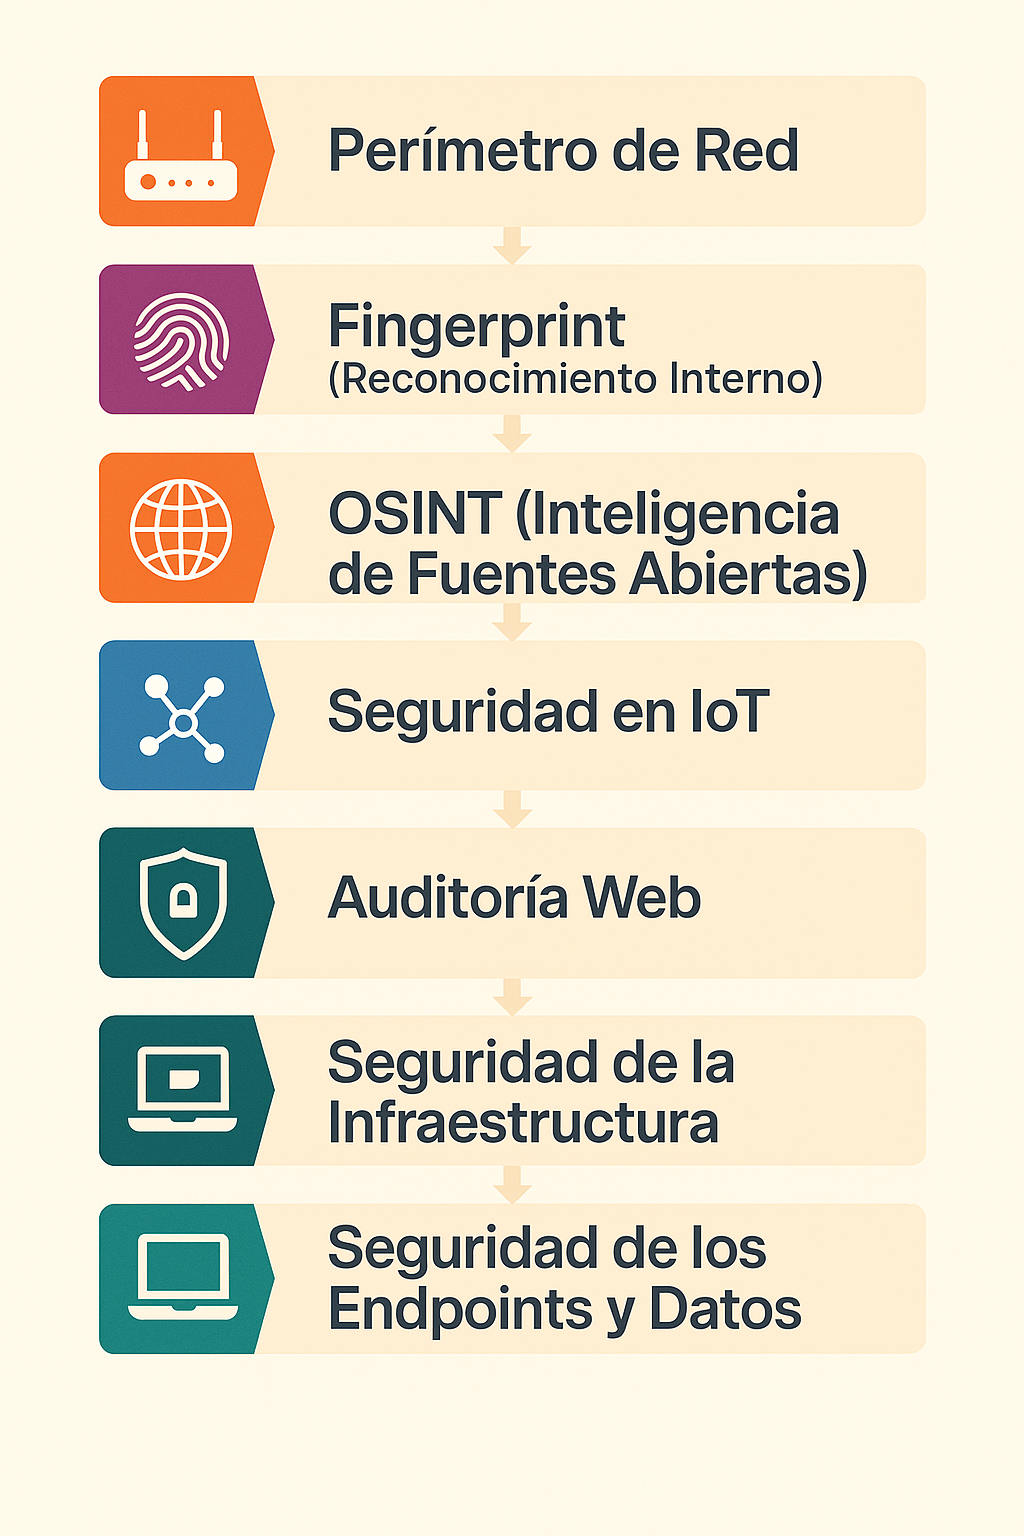
\includegraphics[width=0.45\textwidth]{images/diseno.png}
    \caption{Diagrama de flujo de los bloques del diseño del modelo de auditoría. Fuente: Elaboración propia}
    \label{fig:diseno_modelo_auditoria}
\end{figure}

\begin{enumerate}
    \item \textbf{Perímetro de Red:} Se analiza la exposición externa de la infraestructura desde la perspectiva de un atacante sin conocimiento previo. Se evalúan routers con configuraciones por defecto (telnet, SSH abiertos), firewalls mal configurados, accesos remotos sin cifrado, y redes inalámbricas vulnerables. Se incluyen pruebas sobre sistemas RADIUS, bypass de portales cautivos, detección de APs maliciosos (Rogue AP / Karma WiFi), análisis de seguridad inalámbrica y cifrado.

\item \textbf{Fingerprint (Reconocimiento Interno):} Se realiza un reconocimiento de red interno: análisis de la topología de red, detección activos en la red, enumeración de puertos abiertos y servicios activos en cada activo. 
El mapeo de red se complementa con un análisis de vulnerabilidades.

\item \textbf{OSINT (Inteligencia de Fuentes Abiertas):} Se recopila y analiza información pública sobre la organización para descubrir posibles vectores de ataque. Se utilizan motores como Google (GHDB), Shodan, Censys y Maltego para identificar servidores expuestos, credenciales filtradas, tecnologías empleadas y datos personales. Además, se evalúan técnicas de ingeniería social como phishing.

\item \textbf{Seguridad en IoT:} Dado que muchas pymes incorporan dispositivos inteligentes como cámaras, sensores, esta fase analiza posibles accesos no autorizados a través de estos dispositivos, los cuales suelen estar poco protegidos. Se revisa su firmware, autenticación, cifrado y su exposición en la red.
\item \textbf{Auditoría Web:} Se realizan pruebas de seguridad siguiendo las recomendaciones de OWASP. 

\item \textbf{Seguridad de Infraestructura:} Se revisa la arquitectura interna de la empresa: servidores, redes privadas, Active Directory, firewalls internos, y sistemas IDS/IPS. Se ejecutan pruebas de escalada de privilegios, pivoting, análisis de red, y se evalúa la configuración segura de cada elemento. También se estudian los logs y mecanismos de monitoreo, identificando posibles brechas de seguridad.

\item \textbf{Seguridad de Endpoints y Datos:} Se analiza la protección de los dispositivos finales utilizados por los empleados, donde suele recaer una parte crítica de la seguridad. Se auditan políticas de contraseñas, cifrado de disco, control de dispositivos USB, protección frente a malware, uso de software legítimo, backup de información, y sistemas de almacenamiento.

\end{enumerate}

































































\clearpage

\subsection{Propuesta de auditoría}

En esta sección se describen de forma detallada los distintos bloques que conforman el diseño de la auditoría de seguridad. Se definen los objetivos, herramientas 
y metodología a seguir en cada uno de ellos. Además, se especifican los resultados esperados al finalizar cada bloque para asegurar la correcta implementación del modelo y sus posibles limitaciones
 dentro del entorno empresarial.


\subsubsection{Análisis del Perímetro de Red}

Con el análisis del perímetro de red, intentamos identificar los puntos débiles de la infraestructura desde la perspectiva de un atacante externo, sin conocimiento de la arquitectura interna.

\begin{table}[H]
    \centering
    \renewcommand{\arraystretch}{1.4}
    \begin{tabular}{|p{1.2cm}|p{3.9cm}|p{5.3cm}|p{4.2cm}|}
    \hline
    \textbf{ID} & \textbf{Objetivo} & \textbf{Actividades} & \textbf{Herramientas}\\
    \hline
    OBJ-01 & Detectar redes inalámbricas disponibles & Enumeración de SSIDs visibles y ocultos & Airodump-ng, Wireshark\\
    \hline
    OBJ-02 & Evaluar seguridad de cifrado WiFi & Identificar tipo de cifrado (WEP/WPA/WPA2/Enterprise) captura de handshake & Airodump-ng, hcxdumptool, Aircrack-ng \\
    \hline
    OBJ-03 & Realizar ataques de fuerza bruta a redes inseguras & Diccionario sobre handshake capturado & Aircrack-ng, hashcat \\
    \hline
    OBJ-04 & Validar seguridad de portal cautivo & Intento de bypass (DNS spoof, phishing, MitM) & Bettercap, mitmproxy, macchanger\\
    \hline
    OBJ-05 & Simular Rogue AP y ataques Karma & Clonado de SSID, AP falso para interceptar clientes & WiFi Pineapple, Hostapd, EvilTrust \\
    \hline
    OBJ-06 & Detectar APs mal configurados o sospechosos & Escaneo de redes abiertas, SSID duplicados, canales raros & Airodump-ng, Wireshark\\
    \hline
    OBJ-07 & Identificar routers con credenciales por defecto & Prueba de acceso a SSH, Telnet, interfaces web & Nmap, Hydra \\
    \hline
    \end{tabular}
    \caption{Tabla de trazabilidad de objetivos en el análisis del perímetro de red}
    \end{table}
    

\paragraph{Resultados esperados:}
\begin{itemize}
    \item Inventario de redes inalámbricas detectadas (visibles y ocultas), con información detallada sobre SSID, canal, BSSID (OBJ-01, OBJ-06).
    \item Diagnóstico del tipo de cifrado implementado en cada red, con identificación de aquellas que presenten algoritmos débiles o configuraciones inseguras (OBJ-02).
    \item Registro de contraseñas vulneradas mediante fuerza bruta, con indicación del tiempo estimado (OBJ-03).
    \item Evidencias de portales cautivos vulnerables ante técnicas de evasión o manipulación del tráfico (OBJ-04).
    \item Clientes conectados a AP falsos y evaluación del impacto potencial del ataque mediante Rogue AP o Karma (OBJ-05).
    \item Listado de routers o dispositivos accesibles remotamente con interfaces mal protegidas o credenciales por defecto (OBJ-07).
    \item Recomendaciones específicas de mitigación para cada vulnerabilidad detectada.
\end{itemize}

\paragraph{Limitaciones:}
\begin{itemize}
    \item El análisis externo puede verse obstaculizado por la presencia de firewalls avanzados, WAFs, mecanismos de bloqueo o listas blancas, que filtran escaneos o conexiones sospechosas (OBJ-07).
    \item La detección de redes ocultas depende de la presencia activa de clientes conectados; de no haber tráfico asociado, podrían no identificarse (OBJ-01, OBJ-06).
    \item Las pruebas de fuerza bruta pueden requerir tiempos prolongados y recursos computacionales considerables, lo que limita su viabilidad en escenarios reales (OBJ-03).
    \item Algunas herramientas utilizadas en pruebas como Rogue AP o ataques MitM requieren hardware específico y tráfico en la red. (OBJ-05, OBJ-04).
    \item El uso de técnicas intrusivas, como la simulación de APs maliciosos o la manipulación del portal cautivo, debe realizarse en entornos controlados, ya que podrían provocar interrupciones en la conectividad de usuarios reales si se ejecutan en producción.
    \item La legalidad de determinadas técnicas puede requerir una autorización explícita del cliente antes de su ejecución, especialmente aquellas que simulan comportamiento malicioso (phishing, suplantación, bypass).
\end{itemize}


\clearpage

\subsubsection{Fingerprint y Reconocimiento Interno}

Una vez dentro de la red, se analizan los diferentes dispositivos conectados y sus diferentes vulnerabilidades, para trazar un plan de ataque.

\begin{table}[H]
\centering
\renewcommand{\arraystretch}{1.4}
    \begin{tabular}{|p{1.2cm}|p{3.9cm}|p{5.3cm}|p{4.2cm}|}
\hline
\textbf{ID} & \textbf{Objetivo} & \textbf{Actividades} & \textbf{Herramientas}  \\
\hline
OBJ-08 & Mapeo de la red interna & Descubrimiento de dispositivos, gateways, rutas, subredes & Nmap, Neptus  \\
\hline
OBJ-09 & Análisis de puertos abiertos & Escaneo de red interna, detección de servicios accesibles & Nmap, Masscan, Neptus  \\
\hline
OBJ-10 & Identificación de servicios y versiones & Fingerprinting de servicios, banner grabbing, OS detection & Nmap, WhatWeb, Netcat  \\
\hline
OBJ-11 & Detección de vulnerabilidades conocidas & Escaneo de CVEs, servicios sin parches, versiones antiguas & Nessus, Exploit-db, WhatWeb  \\
\hline

\end{tabular}
\caption{Tabla de trazabilidad de objetivos en la fase de Fingerprint interno}
\end{table}



\paragraph{Resultados esperados:}
\begin{itemize}
    \item Topología detallada de la red interna, con identificación de dispositivos, gateways, y subredes (OBJ-08).
    \item Listado exhaustivo de puertos abiertos y servicios en cada host, con indicación del tipo de protocolo (OBJ-09).
    \item Información precisa sobre los servicios activos, versiones detectadas y sistemas operativos (OBJ-10).
    \item Inventario de vulnerabilidades conocidas asociadas a los servicios detectados, incluyendo identificadores CVE y criticidad (OBJ-11).
    \item Priorización de dispositivos críticos o mal configurados que puedan servir como vectores de escalada o pivoting.
\end{itemize}

\paragraph{Limitaciones:}
\begin{itemize}
    \item La ejecución de escaneos internos requiere acceso a la red local, lo cual puede estar fuera del alcance del auditor en ciertas condiciones (OBJ-08–11).
    \item Las herramientas de escaneo pueden generar falsos positivos o negativos debido a la presencia de firewalls internos, IDS/IPS, o configuraciones personalizadas de los servicios (especialmente en OBJ-09 y OBJ-10).
    \item En redes grandes o mal segmentadas, los tiempos de escaneo aumentan significativamente, lo que puede limitar la cobertura o el rendimiento de las herramientas utilizadas (OBJ-08).
\end{itemize}
\clearpage

\subsubsection{OSINT e Ingeniería Social}

Esta fase se centra en la obtención de información utilizando fuentes abiertas (Open Source Intelligence), recopilando datos públicos que puedan ser útiles para identificar vectores de ataque antes de cualquier interacción directa con los sistemas. Se complementa con técnicas de ingeniería social para evaluar el factor humano.

\begin{table}[H]
\centering
\renewcommand{\arraystretch}{1.4}
    \begin{tabular}{|p{1.2cm}|p{3.9cm}|p{5.3cm}|p{4.2cm}|}
\hline
\textbf{ID} & \textbf{Objetivo} & \textbf{Actividades} & \textbf{Herramientas}  \\
\hline
OBJ-12 & Recolectar información de buscadores genéricos & Búsquedas avanzadas con dorks, índice de documentos, paneles expuestos & Google, Google Hacking DB (GHDB)  \\
\hline
OBJ-13 & Identificar activos expuestos & Recolección de IPs públicas, puertos y servicios accesibles & Shodan, Censys  \\
\hline
OBJ-14 & Analizar relaciones y metadatos en redes y dominios & Investigación de nombres, emails, metadatos de documentos y relaciones entre entidades & Maltego, theHarvester, Recon-ng  \\
\hline
OBJ-15 & Buscar credenciales filtradas y contraseñas públicas & Consultas sobre leaks, validación de emails y dominios comprometidos & DeHashed, HaveIBeenPwned  \\
\hline
OBJ-16 & Evaluar la respuesta humana frente a ataques simulados & Pruebas de phishing, manipulación, evaluación de políticas internas  & GoPhish, RubberDucky \\
\hline
\end{tabular}
\caption{Tabla de trazabilidad de objetivos en la fase OSINT e Ingeniería Social}
\end{table}





\paragraph{Resultados esperados:}
\begin{itemize}
    \item Identificación de documentos, paneles de administración u otros recursos accesibles desde motores de búsqueda mediante el uso de dorks avanzados (OBJ-12).
    \item Inventario de activos públicos expuestos (direcciones IP, puertos, servicios abiertos), con detalles sobre su localización (OBJ-13).
    \item Mapas de relaciones entre dominios, cuentas de correo, nombres de empleados o entidades asociadas, así como metadatos incrustados en documentos (OBJ-14).
    \item Listado de credenciales potencialmente comprometidas, asociadas a dominios corporativos o emails internos (OBJ-15).
    \item Evaluación de la resiliencia del personal frente a técnicas de ingeniería social (OBJ-16).
\end{itemize}

\paragraph{Limitaciones:}
\begin{itemize}
    \item La información obtenida mediante OSINT puede estar desactualizada, parcial o haber sido ya mitigada por la organización en el momento del análisis (OBJ-12–15).
    \item Las herramientas de búsqueda tienen limitaciones en cuanto al alcance de indexación, especialmente en contenidos dinámicos, servicios protegidos o entornos internos no expuestos (OBJ-12, OBJ-13).
    \item La interpretación de relaciones en herramientas como Maltego o Recon-ng puede generar asociaciones erróneas si no se valida manualmente el contexto (OBJ-14).
    \item Las pruebas de ingeniería social requieren autorización explícita y un entorno controlado. Además, su ejecución puede estar condicionada por la normativa laboral y la cultura organizativa de la empresa (OBJ-16).
\end{itemize}

\subsubsection{Seguridad en IoT}

Los dispositivos IoT suelen carecer de medidas de seguridad sólidas y se convierten en vectores frecuentes de ataque. Esta fase se enfoca en el análisis del tráfico de red, servicios inseguros, firmware, y protocolos específicos utilizados por dispositivos conectados.

\begin{table}[H]
\centering
\renewcommand{\arraystretch}{1.4}
    \begin{tabular}{|p{1.2cm}|p{3.9cm}|p{5.3cm}|p{4.2cm}|}
\hline
\textbf{ID} & \textbf{Objetivo} & \textbf{Actividades} & \textbf{Herramientas}  \\
\hline
OBJ-17 & Identificar dispositivos IoT en la red & Escaneo de red, fingerprinting de fabricantes, búsqueda de dispositivos por MAC y puertos comunes & Nmap, Wireshark  \\
\hline
OBJ-18 & Analizar protocolos IoT y tráfico de red & Captura y análisis de paquetes en protocolos propietarios (MQTT, CoAP, BLE, UPnP) & Wireshark  \\
\hline
OBJ-19 & Evaluar la seguridad de interfaces y APIs & Inspección de endpoints HTTP, comandos remotos, autenticación débil o inexistente & Postman, Burp Suite  \\
\hline
OBJ-20 & Detectar firmware inseguro o mal configurado & Extracción y análisis de firmware, validación de backdoors y servicios inseguros & Wireshark  \\
\hline
OBJ-21 & Atacar dispositivos vulnerables & Explotación de servicios abiertos, contraseñas por defecto, ejecución remota de comandos & Metasploit, hydra, scripts personalizados  \\
\hline
\end{tabular}
\caption{Tabla de trazabilidad de objetivos en la auditoría de dispositivos IoT}
\end{table}

\paragraph{Resultados esperados:}
\begin{itemize}
    \item Inventario detallado de dispositivos IoT detectados en la red, con su identificación por fabricante, modelo y dirección MAC (OBJ-17).
    \item Análisis del tráfico de red IoT, con detección de protocolos inseguros, datos transmitidos en texto plano o configuraciones por defecto (OBJ-18).
    \item Evaluación del nivel de exposición de las APIs o paneles de gestión, incluyendo endpoints sin autenticación, tokens expuestos o comandos inseguros (OBJ-19).
    \item Extracción exitosa y análisis estático de firmware, con identificación de puertas traseras, claves embebidas, certificados obsoletos o servicios inseguros habilitados (OBJ-20).
    \item Demostración controlada de vulnerabilidades explotables, como ejecución remota de comandos, credenciales por defecto y escalada de privilegios (OBJ-21).
    \item Recomendaciones específicas de mitigación para cada dispositivo vulnerable o mal configurado.
\end{itemize}

\paragraph{Limitaciones:}
\begin{itemize}
    \item Muchos dispositivos IoT no responden a técnicas de escaneo convencionales o emplean protocolos inusuales, lo que dificulta su identificación (OBJ-17, OBJ-18).
    \item El análisis de tráfico requiere que los dispositivos estén activos y generen comunicaciones durante el período de captura, de lo contrario, ciertos vectores podrían pasar desapercibidos (OBJ-18).
    \item La extracción de firmware puede no ser posible sin acceso físico al dispositivo o sin credenciales propietarias del fabricante, lo que limita la evaluación completa de vulnerabilidades (OBJ-20).
    \item La explotación directa puede ser peligrosa si se realiza en un entorno de producción, pudiendo provocar bloqueos, reinicios o corrupción del sistema (OBJ-21).
\end{itemize}

\subsubsection{Auditoría Web}

En esta fase se analiza por completo la plataforma web, partiendo desde el propio servidor donde se aloja. Se siguen los pasos establecidos por la metodología OWASP para detectar las vulnerabilidades más críticas.

\begin{table}[H]
\centering
\renewcommand{\arraystretch}{1.4}
\begin{tabular}{|p{1.2cm}|p{4cm}|p{4.8cm}|p{3.8cm}|p{2.5cm}|}
\hline
\textbf{ID} & \textbf{Objetivo} & \textbf{Actividades} & \textbf{Herramientas}  \\
\hline
OBJ-22 & Analizar el servidor web y servicios asociados & Fingerprinting, detección de versiones, servicios activos, configuración & WhatWeb, Nikto, Nmap scripts  \\
\hline
OBJ-23 & Identificar servicios vulnerables o expuestos & Enumeración de directorios, endpoints, tecnologías utilizadas & Dirb, Gobuster, Wappalyzer  \\
\hline
OBJ-24 & Detectar vulnerabilidades OWASP & SQLi, XSS, IDOR, RCE, SSRF, CSRF, XXE, etc. & Burp Suite, gestores de contenido \\
\hline
OBJ-25 & Validar mecanismos de autenticación & Fuerza bruta, evasión de login, análisis de formularios & Hydra, Burp Intruder, wfuzz, GoBuster  \\
\hline
OBJ-26 & Evaluar la gestión de sesiones & Análisis de cookies, tokens, regeneración y caducidad de sesiones &  Burp Suite  \\
\hline
OBJ-27 & Probar mecanismos de autorización & Escalada de privilegios, acceso a funciones restringidas & Burp Suite, Postman \\
\hline
OBJ-28 & Validar controles de entrada/salida & Pruebas de validación del lado cliente y servidor, bypasses comunes & Burpsuite, payloads manuales  \\
\hline
OBJ-29 & Explorar la aplicación (crawling/spidering) & Recolección automatizada de rutas y formularios & Burpsuite \\
\hline
OBJ-30 & Realizar fuerza bruta y fuzzing sobre parámetros & Testeo de inputs, formularios & wfuzz, Burpsuite, sqlmap  \\
\hline
OBJ-31 & Evaluar la criptografía usada en la aplicación & Análisis de algoritmos de hash, cifrados, tokens y secretos & Burp Crypto  \\
\hline
\end{tabular}
\caption{Tabla de trazabilidad de objetivos en la auditoría de aplicaciones web}
\end{table}



\paragraph{Resultados esperados:}
\begin{itemize}
    \item Identificación de versiones del servidor web y servicios expuestos, con posibles configuraciones inseguras (OBJ-22).
    \item Descubrimiento de rutas ocultas, endpoints sensibles y tecnologías potencialmente vulnerables (OBJ-23, OBJ-29).
    \item Detección de vulnerabilidades OWASP (como SQLi, XSS, CSRF, etc.), clasificadas según nivel de criticidad (OBJ-24).
    \item Evidencia de fallos en los mecanismos de autenticación, como contraseñas débiles, formularios vulnerables o bypasses de login (OBJ-25).
    \item Análisis de sesiones inseguras: cookies sin flags de seguridad, tokens sin caducidad, falta de regeneración en login/logout (OBJ-26).
    \item Accesos indebidos o escaladas de privilegio mediante manipulación de permisos o tokens de autorización (OBJ-27).
    \item Pruebas de validación inadecuada de entrada/salida que permitan inyecciones o manipulaciones en el flujo de datos (OBJ-28, OBJ-30).
    \item Evaluación de la criptografía utilizada, identificando algoritmos inseguros o mal implementados en la gestión de contraseñas, tokens o almacenamiento (OBJ-31).
    \item Recomendaciones específicas para cada vulnerabilidad detectada, priorizadas por impacto técnico y facilidad de explotación.
\end{itemize}

\paragraph{Limitaciones:}
\begin{itemize}
    \item Muchas vulnerabilidades solo se manifiestan tras autenticación o en condiciones específicas (estado de sesión, tipo de usuario, datos introducidos), lo que puede limitar la cobertura si no se dispone de credenciales o acceso completo (OBJ-24, OBJ-25, OBJ-27).
    \item Los sistemas con WAF, captcha, rate limiting o mecanismos de detección de automatización pueden bloquear ataques de fuzzing, fuerza bruta o crawling automatizado (OBJ-25, OBJ-29, OBJ-30).
    \item La validación criptográfica se limita a los elementos accesibles desde el frontend (tokens, cookies, headers), sin acceso al código backend o configuración de librerías criptográficas (OBJ-31).
    \item La ejecución de pruebas intrusivas como SQLi o RCE debe realizarse con extremo cuidado en entornos de producción, ya que pueden comprometer la integridad del sistema.
\end{itemize}


\subsubsection{Seguridad de Infraestructura}

Esta fase abarca pruebas sobre el núcleo central de la seguridad en la organización.

\begin{table}[H]
\centering
\renewcommand{\arraystretch}{1.4}
\begin{tabular}{|p{1.2cm}|p{4.2cm}|p{4.8cm}|p{3.8cm}|p{2.3cm}|}
\hline
\textbf{ID} & \textbf{Objetivo} & \textbf{Actividades} & \textbf{Herramientas}  \\
\hline
OBJ-32 & Evaluar configuración del firewall & Identificación de puertos permitidos, pruebas de evasión, reglas de filtrado & Nmap, Scapy, tcptraceroute  \\
\hline
OBJ-33 & Verificar funcionamiento de IDS/IPS & Generación de tráfico sospechoso, análisis de alertas y detección de ataques & Metasploit, Nmap  \\
\hline
OBJ-34 & Analizar seguridad del servidor interno & Revisión de servicios, versiones, credenciales por defecto y vulnerabilidades conocidas & Nmap, Nikto, Nessus  \\
\hline
OBJ-35 & Realizar pruebas sobre Active Directory & Enumeración de usuarios, grupos, GPOs, tickets Kerberos & NetExec, CrackMapExec, Kerbrute, impacket  \\
\hline
OBJ-36 & Analizar tráfico y segmentación de red & Sniffing, detección de redes planas, protocolos en claro, ARP poisoning & Bettercap, Responder, Wireshark, tcpdump  \\
\hline
OBJ-37 & Realizar escalada de privilegios en el entorno & Búsqueda de binarios SUID, permisos mal configurados, exploits locales & GTFOBins, ExploitDB  \\
\hline
OBJ-38 & Ejecutar técnicas de pivoting y movimiento lateral & Conexión a otras redes o máquinas a través de un host comprometido & Chisel, ProxyChains, SSH tunneling, Metasploit  \\
\hline
\end{tabular}
\caption{Tabla de trazabilidad de objetivos en la evaluación de la seguridad de la infraestructura}
\end{table}




\paragraph{Resultados esperados:}
\begin{itemize}
    \item Listado de reglas del firewall efectivas, puertos abiertos innecesariamente o configuraciones que permiten tráfico no autorizado (OBJ-32).
    \item Comprobación del funcionamiento de IDS/IPS ante tráfico anómalo, identificación de firmas activas o ausencia de detección (OBJ-33).
    \item Evaluación de seguridad de servidores internos: servicios inseguros, credenciales por defecto, vulnerabilidades sin parchear (OBJ-34).
    \item Enumeración de la estructura del Active Directory: usuarios, políticas de grupo, servicios Kerberos y relaciones de confianza (OBJ-35).
    \item Detección de segmentación inadecuada en redes mediante análisis de tráfico y técnicas de sniffing (OBJ-36).
    \item Identificación de rutas para escalada de privilegios: binarios mal configurados, exploits locales disponibles y configuraciones débiles (OBJ-37).
    \item Mapeo de movimiento lateral y pivoting: hosts accesibles desde un nodo comprometido, redes internas accesibles sin controles adecuados (OBJ-38).
    \item Recomendaciones de mitigación técnica, incluyendo segmentación, refuerzo de controles de acceso y actualización de servicios vulnerables.
\end{itemize}

\paragraph{Limitaciones:}
\begin{itemize}
    \item La ejecución de pruebas sobre firewall, AD o escalada de privilegios requiere permisos elevados, a menudo restringidos por la política de la organización (OBJ-32, OBJ-35, OBJ-37).
    \item Las técnicas de pivoting y movimiento lateral pueden causar interferencias en la red o en servicios productivos si no se realizan en entornos aislados (OBJ-38).
    \item El análisis de tráfico puede estar limitado por la encriptación de extremo a extremo o el uso de VLANs y redes virtuales que impidan el sniffing pasivo (OBJ-36).
    \item Las herramientas de enumeración como CrackMapExec o Kerbrute pueden generar tráfico considerado agresivo, que puede activar alarmas de IDS o sistemas de bloqueo temporal (OBJ-33, OBJ-35).
    \item La recopilación de logs, políticas de grupo o información sensible del dominio puede estar regulada por normativas internas o leyes de protección de datos, limitando el alcance de algunas técnicas (OBJ-35, OBJ-36).
\end{itemize}


\subsubsection{Seguridad de Endpoints y Datos}

Esta fase se enfoca en los dispositivos cliente de la organización, evaluando su configuración de seguridad, control de accesos, privilegios de usuario, y posibles vectores de evasión de controles mediante proxies, software no autorizado o escaladas locales.
Además, se evalúan un coonjunto de test sobre el almacenamiento de los datos y su sistema de respaldo.
\begin{table}[H]
\centering
\renewcommand{\arraystretch}{1.4}
\begin{tabular}{|p{1.2cm}|p{4.2cm}|p{4.8cm}|p{3.8cm}|p{2.3cm}|}
\hline
\textbf{ID} & \textbf{Objetivo} & \textbf{Actividades} & \textbf{Herramientas}  \\
\hline
OBJ-39 & Evaluar configuración de roles y perfiles de usuario & Verificación de restricciones según rol, acceso a configuraciones y consolas & Manual, PowerShell  \\
\hline
OBJ-40 & Verificar control de puertos USB y dispositivos externos & Comprobación de bloqueo, acceso a discos externos, ejecución automática & USB Rubber Ducky, scripts batch, manual  \\
\hline
OBJ-41 & Intentar escalada local de privilegios & Búsqueda de configuraciones inseguras, binarios vulnerables o mal permisos & ExploitDB, GTFOBins  \\
\hline
OBJ-42 & Comprobar bypass de proxy corporativo & Intento de acceso directo a Internet, uso de túneles y software alternativo & proxychains, TOR, chisel, VPN port forwarding  \\
\hline
OBJ-43 & Instalar y ejecutar software no autorizado & Prueba con aplicaciones portables o autoejecutables desde usuarios limitados & TOR Browser, portable apps, reverse shells  \\
\hline
OBJ-44 & Verificar restricciones sobre terminales y consolas & Evaluar si un perfil básico puede lanzar CMD, PowerShell o interpretes & Terminal  \\
\hline
\end{tabular}
\caption{Tabla de trazabilidad de objetivos en la auditoría de seguridad de endpoints}
\end{table}


\paragraph{Resultados esperados:}
\begin{itemize}
    \item Verificación del cumplimiento de políticas de acceso según perfil de usuario: restricciones adecuadas, acceso limitado a configuraciones del sistema o consolas administrativas (OBJ-39, OBJ-44).
    \item Comprobación del control físico de dispositivos: detección de políticas activas sobre uso de puertos USB, ejecución automática o instalación de drivers externos (OBJ-40).
    \item Identificación de rutas de escalada local mediante binarios inseguros, scripts mal configurados o servicios con permisos excesivos (OBJ-41).
    \item Evidencia de posibles bypasses del proxy corporativo mediante uso de túneles cifrados o canales alternativos de comunicación externa (OBJ-42).
    \item Informe sobre medidas de protección de datos locales y sistemas de backup, incluyendo cifrado de disco, políticas de restauración y almacenamiento redundante.
\end{itemize}

\paragraph{Limitaciones:}
\begin{itemize}
    \item Algunos sistemas de protección avanzados com antivirus pueden interferir en la ejecución de pruebas o generar falsos negativos/positivos (OBJ-41, OBJ-43).
    \item Las pruebas de ejecución de software no autorizado, tunnels o bypasses de proxy pueden entrar en conflicto con políticas internas o requerir una autorización explícita (OBJ-42, OBJ-43).
    \item El análisis de backup o cifrado de disco puede no ser viable sin credenciales administrativas o acceso a la documentación interna de TI (políticas, scripts, logs) (objetivo general).
    \item Las técnicas de evaluación manual pueden depender del entorno operativo (Windows, Linux) y requerir enfoques diferenciados para cada uno.
\end{itemize}


\clearpage

























\subsection{Metodología de auditoría}

La auditoría se llevará a cabo mediante una metodología híbrida que combina enfoques \textbf{White Box} (con conocimiento previo de la estructura interna) y \textbf{Grey Box} (con acceso parcial), simulando escenarios realistas como los que podrían surgir en ataques internos o a través de empleados con conocimientos limitados pero con acceso legítimo.

\par\vspace{0.5cm}
Las fases metodológicas que se aplicarán durante la auditoría son:

\begin{enumerate}
\item \textbf{Planificación:} Definición del alcance, recursos disponibles, cronograma, responsables y objetivos específicos. Se documenta el entorno inicial y se establecen los límites éticos y técnicos de la auditoría.

\item \textbf{Reconocimiento y Enumeración:} Se realiza un análisis exhaustivo del entorno mediante diversos escaneos, aplicando técnicas previamente definidas de \textit{fingerprinting} interno y externo. Se identifican equipos, servicios activos y puertos abiertos. Adicionalmente, se emplean técnicas de OSINT para recopilar información complementaria. Todos los datos obtenidos se documentan detalladamente.

\item \textbf{Evaluación de Seguridad:} Ejecución práctica de las pruebas definidas en la propuesta. Se documentan vulnerabilidades, configuraciones inseguras, errores de diseño, exposición innecesaria y carencias organizativas.

\item \textbf{Análisis de Riesgos:} Se evalúa la probabilidad de explotación de cada hallazgo, su impacto sobre el negocio y la posibilidad de encadenar vulnerabilidades. Se aplica una matriz de criticidad y se priorizan riesgos.

\item \textbf{Informe Final:} Se elabora un documento técnico con todos los hallazgos, acompañado de evidencias, explicación de riesgos, herramientas utilizadas, niveles de criticidad, y recomendaciones de mejora.

\end{enumerate}


\clearpage




% -----------------------------------------------CASO PRÁCTICO------------------------------------------------------------
\section{Caso Práctico}

\subsection{Implementación de la auditoría}

La auditoría fue llevada a cabo en colaboración con el equipo profesional de \textbf{BeeHacker}, aplicando el modelo metodológico híbrido definido previamente, 
que combina enfoques \textbf{White Box} y \textbf{Grey Box}. 

\par\vspace{0.4cm}

El entorno auditado corresponde a una \textbf{pyme del sector industrial} ubicada en territorio nacional. Por motivos de confidencialidad y conforme a los principios éticos 
establecidos en la fase de planificación, se ha optado por mantener el anonimato de la entidad analizada, la cual será referida en este documento como \textbf{Empresa X}. 
\par\vspace{0.4cm}

Además, se utilizarán nombres de dominio ficticios para proteger la identidad de los sistemas y aplicaciones involucradas, evitando así cualquier posible asociación con la empresa real. Asimismo, la direcciones IP públicas y nombres de host utilizados durante la práctica serán también ficticios y no corresponden a sistemas reales.

\par\vspace{0.4cm}

La auditoría se estructuró conforme a las cinco fases metodológicas descritas en el capítulo anterior:

\begin{itemize}
    \item En la \textbf{fase de planificación}, se delimitaron los activos objeto de análisis, incluyendo infraestructura de red, servidores, endpoints, dispositivos IoT y la aplicación web corporativa. Se firmaron acuerdos de confidencialidad y se definieron las condiciones bajo las cuales se podían ejecutar ataques controlados.
    
    \item Durante la \textbf{fase de reconocimiento y enumeración}, se realizó una recolección de información tanto externa como interna. Se aplicaron técnicas OSINT, escaneos de red, análisis de puertos y fingerprinting para identificar la superficie de ataque visible desde distintos puntos.
    
    \item En la \textbf{fase de evaluación de seguridad}, se ejecutaron las pruebas planificadas para cada uno de los vectores establecidos: red perimetral, infraestructura interna, dispositivos IoT, aplicación web, políticas de endpoints, y respuesta ante ingeniería social. Todas las actividades se realizaron bajo supervisión y sin afectar la continuidad operativa de la empresa.
    
    \item En la \textbf{fase de análisis de riesgos}, los hallazgos fueron evaluados según su impacto potencial y probabilidad de explotación. Se elaboró una matriz de criticidad que permitió priorizar las vulnerabilidades según su riesgo real para el negocio.
    
    \item Finalmente, en la \textbf{fase de elaboración del informe}, se entregó un documento técnico estructurado que incluye: hallazgos, evidencias gráficas, análisis de riesgos, herramientas utilizadas y un conjunto de recomendaciones clasificadas por urgencia e impacto.
\end{itemize}

\par\vspace{0.4cm}






\clearpage

% -----------------------------------------------RESULTADOS------------------------------------------------------------
\section{Resultados}



\clearpage

% -----------------------------------------------CONCLUSIONES O DISCUSIONES------------------------------------------------------------
\section{Conclusiones}



\clearpage

% -----------------------------------------------REFERENCIAS------------------------------------------------------------
%Poner bien las referencias en APA, en word puedo crear las bibliografias ya sean de entrevistas a empresas, webs, articulos... Se citan  \cite{farlopa} en el código para un ajuste final de la bibliografía.
\begin{thebibliography}{20}
    
    \bibitem{farlopa}
    DefSec. (s.f.). \textit{Mariscada virtual en el servidor de CCOO}. Recuperado el 08 de febrero de 2025, de \url{https://defsec.noblogs.org/mariscada-virtual-en-el-servidor-de-ccoo/}
    
    \bibitem{avtest}
    AV-TEST. (s.f.). \textit{AV-Atlas Malware Portal}. Recuperado el 10 de enero de 2025, de \url{https://portal.av-atlas.org/malware}
    
    \bibitem{mitigacion}
    Por Alguien. (2222) \url{http://perspectivas.espoch.edu.ec:8081/index.php/RCP_ESPOCH/article/view/215/146 consultado el 5/5/2025}
    
    \bibitem{agencia_digital} 
    Agencia Digital de Andalucía. (2024). \textit{Documento de transparencia sobre costes laborales en perfiles TIC}. Encontrado el 13 de febrero de 2025, de \url{https://ws040.juntadeandalucia.es/webconsejos/cgobierno/transparencia/240730/documentos/30Expediente.pdf}
    
    \bibitem{vuln}
    Morales-López \& Taipe-Yanez \& Pallo-Tulmo, (2024) \textit{Estrategias de Auditoría en ciberseguridad y su importancia en las empresas una revisión bibliográfica} Encontrado el 07 de abril de 2025 de \url{https://www.investigarmqr.com/ojs/index.php/mqr/article/view/1436/4849}

    \bibitem{boe}
    Boletín Oficial del Estado. (2024). Código Electrónico de Ciberseguridad. el 08 de abril de 2025 Recuperado de: \url{https://www.boe.es/biblioteca_juridica/codigos/codigo.php?id=173}

    \bibitem{cadena_ser}
    Cadena SER. (2024). ¿Qué cambia la directiva de la UE que mejora la ciberseguridad y ya aplican los Estados?. el 08 de abril de 2025 Recuperado de: \url{https://cadenaser.com/cmadrid/2024/10/22/que-cambia-la-directiva-de-la-ue-que-mejora-la-ciberseguridad-y-ya-aplican-los-estados-ser-madrid-sur/}

    \bibitem{bce}
    Banco Central Europeo. (2025). Decisiones adoptadas por el Consejo de Gobierno del BCE. el 08 de abril de 2025 Recuperado de: \url{https://www.ecb.europa.eu/press/govcdec/otherdec/2025/html/ecb.gc250131~d2c6d582b0.es.html}

    \bibitem{comision_europea}
    Comisión Europea. (2023). Una Europa Adaptada a la Era Digital. Recuperado de:el 08 de abril de 2025  \url{https://commission.europa.eu/strategy-and-policy/priorities-2019-2024/europe-fit-digital-age_es}

    \bibitem{escudo2023}
    Escudo Digital. (2023). INCIBE, CNI y CCN se reúnen para impulsar su coordinación en ciberseguridad. Recuperado de: \url{https://www.escudodigital.com/ciberseguridad/incibe-cni-ccn-se-reunen-impulsar-su-coordinacion-en-ciberseguridad_54930_102.html}

    \bibitem{felipe2024}
    Felipe Redondo, A. M., \& Núñez Cárdenas, F. J. (2024). \textit{Criterios de selección de herramientas para pentesting}. Ciencia Huasteca Boletín Científico de la Escuela Superior de Huejutla, 12(24), 31-35. Recuperado de \url{https://repository.uaeh.edu.mx/revistas/index.php/huejutla/article/view/12763/11251}
    
    \bibitem{hiscox}
    Hiscox (2022). \textit{ 44\% de las pymes españolas sufrió al menos un ciberataque durante 2021} Recuperado de \url{https://www.hiscox.es/el-44-de-las-pymes-espanolas-sufrio-al-menos-un-ciberataque-durante-2021}

    \bibitem{incibe2023}
    INCIBE (2023). \textit{INCIBE gestionó más de 118.000 incidentes de ciberseguridad durante 2022, un 9\% más que en 202} Recuperado de \url{https://www.incibe.es/incibe/sala-de-prensa/incibe-gestiono-mas-115000-incidentes-ciberseguridad-durante-2022-9-mas}

    \bibitem{pow}
    POW (2021). \textit{El 86\% de las compañías españolas carecen de una cultura de ciberseguridad entre los empleados} Recuperado de \url{https://www.pwc.es/es/sala-prensa/notas-prensa/2021/companias-espanolas-cultura-ciberseguridad-empleados.html}

    \bibitem{toms2021}
    Toms, L. (2021). \textit{5 riesgos de seguridad para las PYMEs que se deben tener en cuenta} Recuperado de \url{https://www.globalsign.com/es/blog/top-5-pequena-empresa-grandes-riesgos-5-riesgos-de-seguridad-para-las-pymes-que-se-deben-tener-en-cuenta}
    
    \bibitem{treider}
    Treider, A. (2021). \textit{Ciberseguridad para pymes: ¿Por qué es importante?} Recuperado del 07 de abril \url{https://www.treyder.com/blog/ciberseguridad-en-las-pymes/}
\end{thebibliography}


\clearpage







% -----------------------------------------------ANEXOS------------------------------------------------------------
\section{Anexos}

\begin{table}[H]
\centering
\begin{tabular}{|p{4cm}|p{8cm}|}
\hline
\textbf{Herramienta} & \textbf{URL de referencia / descarga} \\
\hline
Kali Linux & \url{https://www.kali.org} \\
Parrot OS & \url{https://www.parrotsec.org} \\
Nmap & \url{https://nmap.org} \\
Nessus & \url{https://www.tenable.com/products/nessus} \\
OpenVAS & \url{https://www.greenbone.net/en/} \\
Nikto & \url{https://github.com/sullo/nikto} \\
SQLMap & \url{https://sqlmap.org} \\
Burp Suite & \url{https://portswigger.net/burp} \\
OWASP ZAP & \url{https://www.zaproxy.org} \\
Shodan & \url{https://www.shodan.io} \\
Censys & \url{https://censys.io} \\
TheHarvester & \url{https://github.com/laramies/theHarvester} \\
Maltego & \url{https://www.maltego.com} \\
Wireshark & \url{https://www.wireshark.org} \\
Tcpdump & \url{https://www.tcpdump.org} \\
Metasploit & \url{https://www.metasploit.com} \\
BloodHound & \url{https://github.com/BloodHoundAD/BloodHound} \\
CrackMapExec & \url{https://github.com/Porchetta-Industries/CrackMapExec} \\
Mimikatz & \url{https://github.com/gentilkiwi/mimikatz} \\
Flipper Zero & \url{https://flipperzero.one} \\
USB Rubber Ducky & \url{https://shop.hak5.org/products/usb-rubber-ducky-deluxe} \\
Cactus WHID & \url{https://github.com/spacehuhntech/WHID-Injector} \\
\hline
\end{tabular}
\caption{Listado de herramientas utilizadas en auditorías de ciberseguridad y sus referencias oficiales}
\end{table}


\clearpage



\end{document}